\documentclass[11pt,a4paper,openany]{book}

%\usepackage[german]{babel}	%in case you want to write a german thesis

%settings for generation of titlepage, index and table of content
\usepackage{graphicx}
\usepackage{geometry}
\usepackage{fancyhdr}
\usepackage{tabularx}
\usepackage[
indexing=cite,
backend=biber,
sorting=nyt,
maxcitenames=1, 
mincitenames=1, 
maxbibnames=999, 
minbibnames=999,
refsection=section,
autocite=footnote,
doi=true,
url=true,
style=authortitle-ibid
]{biblatex}
\usepackage{makecell}
\usepackage{titlesec}
\usepackage{lipsum}
\usepackage[super]{nth}
\usepackage{imakeidx}
\usepackage{hyperref}
\usepackage{listings}
\usepackage{color}
\usepackage{footnote}
\usepackage{amsmath}


\definecolor{dkgreen}{rgb}{0,0.6,0}
\definecolor{gray}{rgb}{0.5,0.5,0.5}
\definecolor{mauve}{rgb}{0.58,0,0.82}
\definecolor{orange}{RGB}{255,143,0}
\definecolor{dkblue}{rgb}{0.14, 0.13, 0.35}
\definecolor{brown}{rgb}{0.321, 0.105, 0.113}

\lstset{frame=tb,
	language=python,
	aboveskip=5mm,
	belowskip=5mm,
	showstringspaces=false,
	columns=flexible,
	basicstyle={\small\ttfamily},
	numbers=left,
	numberstyle=\tiny\color{gray},
	keywordstyle=\color{orange},
	commentstyle=\color{dkgreen},
	stringstyle=\color{mauve},
	breaklines=true,
	breakatwhitespace=false,
	tabsize=4
}

\pagestyle{fancy}
\fancyhf{}
\setlength{\headheight}{45pt}

\lhead{
  
\includegraphics[width=3cm]{img/htlwrn_logo}  
}
\chead{\Large HTBLuVA Wiener Neustadt \\ \normalsize Höhere Lehranstalt für Informatik}
\rhead{
  
\includegraphics[width=3cm]{img/htlwrn_logo2}
}

\newcommand{\parseauthor}[3]{\makecell{#1 \\ #2} & & #3}

\def \title {\Huge \bf D\,I\,P\,L\,O\,M\,A\,R\,B\,E\,I\,T}

\setlength{\parindent}{0em}

\geometry{
 a4paper,
 left=30mm,
 top=50mm,
 }
 
\graphicspath{ {img/} }

\makeindex[title=Index]
\makeindex[name=allgemein, title=Common Index]
\makeindex[name=name,title={Authors Index}]
	% do not even think about changing this from name to author
\makeindex[name=title,columns=1,title={Literature Index}]
\indexsetup{level=\subsection*, toclevel=subsection, noclearpage}


\makeatletter
\@ifpackageloaded{biblatex_legacy}
{\DeclareIndexNameFormat{default}{%
		\usebibmacro{index:name}{\index[name]}{#1}{#3}{#5}{#7}}}
{\DeclareIndexNameFormat{default}{%
		\usebibmacro{index:name}{\index[name]}
		{\namepartfamily}
		{\namepartgiven}
		{\namepartprefix}
		{\namepartsuffix}}}
\makeatother

\DeclareIndexFieldFormat{indextitle}{%
	\usebibmacro{index:title}{\index[title]}{#1}}

\renewbibmacro*{bibindex}{%
	\ifbibindex
	{\indexnames{author}%
		\indexnames{editor}%
		\indexnames{translator}%
		\indexnames{commentator}%
		\indexfield{indextitle}}
	{}}

\makeatletter
\DeclareCiteCommand{\repeatfootcite}[\cbx@wrap]
{\gdef\cbx@keys{}}
{\xappto\cbx@keys{\thefield{entrykey},}}
{}
{\ifcsundef{cbx@lastin@\cbx@keys @\strfield{postnote}}
	{\csnumgdef{cbx@lastin@\cbx@keys @\strfield{postnote}}{-1}}{}%
	\ifsamepage{\value{instcount}}{\csuse{cbx@lastin@\cbx@keys @\strfield{postnote}}}
	{\footnotemark[\csuse{cbx@lastfn@\cbx@keys @\strfield{postnote}}]}
	{\xappto\cbx@cite{\noexpand\footcite%
			[\thefield{prenote}][\thefield{postnote}]{\cbx@keys}%
			\csnumgdef{cbx@lastfn@\cbx@keys @\strfield{postnote}}{\value{\@mpfn}}%
			\csnumgdef{cbx@lastin@\cbx@keys @\strfield{postnote}}{\value{instcount}}}}}

\newrobustcmd{\cbx@wrap}[1]{#1\cbx@cite\gdef\cbx@cite{}}
\def\cbx@cite{}
\makeatother

%Messbox zur Druckkontrolle:
\newcommand{\Messbox}[2]{% Parameters: #1=Breite, #2=Hoehe
	\setlength{\unitlength}{1.0mm}%
	\begin{picture}(#1,#2)%
	\linethickness{0.05mm}%
	\put(0,0){\dashbox{0.2}(#1,#2)%
		{\parbox{#1mm}{%
				\centering\footnotesize 
				%{\bf MESSBOX}\\ 
				Breite $ = #1 {\rm\ mm}$\\
				H\"ohe $ = #2 {\rm\ mm}$
	}}}\end{picture}
}

%change hyperref colors
\hypersetup{
	colorlinks = true,
	linkcolor = brown,
	filecolor = blue,
	citecolor = dkblue,      
	urlcolor = dkblue,
}

%suppress visited on ... in footnotes
\AtEveryCitekey{\clearfield{urlyear}}
\AtEveryCitekey{\clearfield{url}}
\AtEveryCitekey{\clearfield{year}}


%definitions for easier costumization
\def \subtitle {Autonomous universal Mapping and Navigation}
\def \year {2020/21}
\def \authors { \parseauthor{Themengebiet 1}{Lukas Leskovar}{5BHIF}\\
                \parseauthor{Themengebiet 2}{Fabian Kleinrad}{5BHIF}}
\def \supervisor {MMag. Dr. Michael Stifter}
\def \declauthors{ Lukas Leskovar & Fabian Kleinrad}	% for two authors
% \def \declauthors{ Vor- und NACHNAME & Vor- und NACHNAME \\ Vor- und NACHNAME}	% for three authors

\addbibresource{main.bib}

\begin{document}
	\pagenumbering{none}
	
	%include titlepage
	\begin{titlepage}
  \thispagestyle{fancy}
  \begin{center}
    \Huge
    \texttt{\textbf{\title}} \\
    \vspace{1cm}
    \LARGE
    \bf{\subtitle}\\
  \end{center}
  \vspace{2cm}
  \begin{flushleft}
    \normalsize
    \textbf{Ausgeführt im Schuljahr \year \ von:}\\
    \vspace{2mm}
     \begin{tabularx}{\linewidth}{lXr}
        \authors
      \end{tabularx} \\
  \end{flushleft}
  \vfill
  \begin{center}
      \vspace{1cm}
      \textbf{Betreuer / Betreuerin:}\\
    \vspace{2mm}
    \begin{tabular}{l}
      \supervisor
    \end{tabular}
    
    \vspace{2cm}
    
    Wiener Neustadt, am 4. April 2022
    
    \rule{14cm}{0.4mm}
    
    \begin{tabular}{p{.4\textwidth}p{.4\textwidth}}
      \scriptsize{Abgabevermerk:} & \scriptsize{Übernommen von:}
    \end{tabular}
    
  \end{center}
\end{titlepage}

	
	%include acknowledgements, abstract and documentation
	
	\pagestyle{plain}
	
%	\frontmatter
	
	\pagenumbering{roman}
	% english word for 'eidestattliche erklärung?'

\chapter{Eidestattliche Erklärung}

\vspace{10mm}

\normalsize
Hiermit erkläre ich an Eides statt, dass ich die vorliegende Arbeit selbstständig und ohne fremde Hilfe verfasst und keine anderen als die im Literaturverzeichnis angegeben Quellen und Hilfsmittel verwendet habe. Insbesondere versichere ich, dass ich alle wörtlichen und sinngemäßen Übernahmen aus anderen Werken als solche kenntlich gemacht habe.

\vspace{1cm}

Wiener Neustadt am 4. April 2022 \\

\vspace{1cm}

{\bf Verfasser:} \\

\renewcommand{\arraystretch}{5}
  \begin{tabular}{p{.4\textwidth}p{.4\textwidth}}
    \declauthors
  \end{tabular}
\renewcommand{\arraystretch}{1}
	
	\tableofcontents
	
	\chapter{Acknowledgement}

First and foremost, the authors would like to thank F-WuTS and robo4you for providing the equipment and facilities used during the development of the Autumn project. Furthermore, we want to thank our supervisor MMag. Dr. Michael Stifter, who's support, motivation and advice were of integral importance for the authors and this thesis.\linebreak

\textbf{Author: Fabian Kleinrad}

My gratitude is due to all the people who have helped me with topic or non-topic specific questions. This made realizing this project possible and directly affected the quality of the outcome. 
Especially I would like to express my thanks to Mag. Michael Krebs for proofreading reading our diploma thesis.

\textbf{Author: Lukas Leskovar}

%This thesis required a lot of effort and motivation. Fabian Kleinrad and his excellent work always pushed me to perform harder than I would've ever been alone. For this, I am very thankful. 

I would also like to thank everyone who read this thesis and contributed insight from a non-technical standpoint, improving its overall quality and readability. 

Most notably, I am very grateful for my family and friends and their support throughout the past five years. 

	\chapter{Kurzfassung}

\vspace{10mm}

Heutzutage unterstützen uns Computer mehr als je zuvor in allen Bereichen unserer Arbeit. Von digital gestürzter Gebäudekonstruktion, bis hin zu Computer basierter Waldwachsbeurteilung. Autumn bietet hierbei eine Lösung, diese Vorhaben durch eine autonome und universell einsetzbare Drohne zu vereinfachen. Die Drohne erstellt ein realitätsnahes 3-D Modell der Umgebung. Dies kann beispielsweise genutzt werden, um Maße zu entnehmen oder eine Momentaufnahme eines Vorhabens festzuhalten. Aufgrund der verwendeten Technologien ist die Drohne unabhängig von äußeren Lokalisierungsmechanismen und kann dadurch in abgelegenen Geländen eingesetzt werden. Realisiert wird dies durch den Einsatz eines SLAM-Algorithmus, um das Mapping zu ermöglichen, und einen RRT* Algorithmus für die Pfadfindung.

\chapter{Abstract}

\vspace{10mm}

Computers nowadays are integrated into a wide variety of processes. Ranging from computer-aided construction to software-based monitoring of forests. Autumn proposes a solution of using an autonomous and universally deployable drone to simplify these tasks. The drone generates a realistic model of the environment, which can be used to extract measurements or capture the momentary progress. Furthermore, autumn uses technologies that enable the drone to work independently of any external localisation mechanism, which allows for deployment in secluded areas. This characteristic can be realised by using a SLAM algorithm, needed to map the environment in combination with an RRT* algorithm, which handles the path-planning.

	
	%include thesis
	
	\mainmatter
	\pagenumbering{arabic}
	
	\chapter{Introduction}

\textbf{Author: Vor- und Nachname}

\vspace{2mm}

\lipsum[1-3]

\section{Section}
More text. \lipsum[1] See Figure~\ref{pic:example}.

\begin{figure}[h]
	\centering
	\includegraphics[width=2.5in]{img/example.png}
	\caption{Picture description.}
	\label{pic:example}
\end{figure}

\subsection{Subsection}
\lipsum[1]

\subsection{Subsection}
\lipsum[1] See Table~\ref{tab:example}.

\begin{center}
	\begin{tabular}{| l | l | l |}
		\hline
		\bfseries Header 1 & \bfseries Header 2 & \bfseries Header 2 \\
		\hline
		Text & text & text \\
		\hline
		Text & text & text  \\
		\hline
		Text & text & text  \\
		\hline
	\end{tabular}
	\label{tab:example}
\end{center}



\lipsum[1] Some references can be found at \footcite{robo4you} or at  \footcite{Hope_Learning_TensorFlow}. 


\filbreak

	\chapter{Study of Literature}

\textbf{Author: } 


\filbreak
	
	\chapter{System Architecture}
\label{chapter:architecture}

\textbf{Author: Lukas Leskovar} 

This chapter aims to provide a thorough overview of Autumns system architecture by describing its construction as well as logical and computational  structure. To this end, the difficulties faced during development and decisions made that affected the overall project are described.

\section{First Prototype}
The first version of the Autumn drone consisted of three main components:
\begin{itemize}
	\item A DJI Matrice 100 functioning as the base of the system powering all external components.
	\item To perform 3D mapping a Stereolabs ZED 1 was mounted onto the lower front part of the drone
	\item As the main component used to compute 3D mapping and control the drone a NVIDIA Jetson TX2 was mounted onto the drones expansion bay.
\end{itemize}
This prototype quickly demonstrated which part of the system needed to be improved where as the main issues were the lack of computational power and usage of non optimal hardware. A detailed explanation as well as a multitude of solutions to this problem are discussed in the following sections.


\section{Processing and power management}
%In the past decades the computational power of microprocessors has dramatically increased to the point where the transistors contained in these processors cannot be built smaller thus limiting the overall computational power.

%In the past decades research has pushed the limits of computational performance of processors further to its limits, all while performing a trade off concerning power requirements. Modern circuits can execute complex algorithms with high speed calculations but therefore have high energy requirements. 
%This confrontation of performance and power is a major issue faced in most robotic applications and therefore affected the implementation of this diploma thesis. In order to perform 3D mapping and local navigation, Autumn requires to execute complex and load heavy algorithms that will be discussed in further detail in later sections. 

In the past decades research has made vast improvements concerning the performance of processors whether they are used as stand-alone microprocessors, microcontrollers, embedded processors or digital signal processors. However these improvements come at the cost of higher power requirements. This trade-off is a major concern in many robotic applications that are powered by batteries or are restricted to low power inputs. Since Autumn is powered only by a drone battery this issue is groundbreaking during the development of this diploma thesis. 

The central component of the system is a NVIDIA Jetson TX2 board equipped with a 2GHz NVIDIA Denver2 dual-core and a 2GHz Arm Cortex-A57 quad-core processor. \footcite{jetsonHardwarePageNoDate}

Using NVIDIA tegrastats \footcite{nvidiaTegrastatsNoDate} the average power consumption of the system at an idle state was measured at 2.7W. However while performing non optimized 3D mapping and navigation algorithms (Chapter \ref{chapter:slam}) with both processors fully utilized and Max-N power mode activated the average power consumption reached 7.9W. \footcite{jetsonPowerModesNoDate} 
%schreib drüber dass diese zahlen bedeuten dass das system komplett ausgelaset ist
Operating the system at such high stress does not only quickly drain the drones battery but also impairs the quality of the resulting 3D map as well as operating the drone.


\section{Solving processing limitations}
When dealing with load heavy computations one way to solve quality issues is to use higher performance hardware, however due to aforementioned power constraints and drone payload requirements this approach is not suitable for this project. 
Another possible solution is to lower the computational load of the processors therefore improving result quality and lowering power consumption. 
This approach was tested in the following two forms:
\begin{itemize}
%	\item Distributing high power computations to a remote host. For most applications out- sourcing computation to a cloud would be the optimal solution however the work en- vironment of Autumn does not allow for a sufficient internet connection. The only possible way to implement this approach was to bring a powerful computer on site and have it wirelessly communicate with the Autumn drone.
	
	\item Distributing high power computations to a remote host. This approach loweres the amount of computation on the drone but requires to use a high performance computer on site to wirelessly communicate with the drone. Furthermore the wifi-range becomes another limiting factor since with increasing range the latency increased thus impairing the result quality again.
	
	\item The second approach was to disable visual odometry using feature extraction and pattern matching as the most complex part of the algorithm and providing odometry using a much more performant visual inertial odometry algorithm. To this end the drone was equipped with a Stereolabs ZED 2i stereo-camera which is benchmarked against other sensors in section \ref{chapter:sensors}%which performed a hardware accelerated sensor-fusion of Inertial Measurement Unit (IMU) Data and visual odometry. %Furthermore the overall mapping quality compared to the Stereolabs ZED 1 was improved due to better depth sensing technology. 
\end{itemize}

\section{Final Product}
Following the aforementioned approach the main causes of performance issues where eliminated by replacing non optimized hardware components and distributing non-critical computations such as user interaction or path planning to a remote host as impairing these aspects of the system by latency would not pose less of a problem. 
With these adjustments the Autumn drones final version consisted of the following altered components:
\begin{itemize}
	\item As already mentioned the Stereolabs ZED 1 was replaced by its successor the Stereolabs ZED 2i. With its additional sensors and out of the box sensor fusion available it greatly reduced the amount of computations performed on the NVIDIA Jetson TX2. 
	\item In order to establish a connection to a remote host and perform computations the Dual Band 2.4GHz and 5GHz Antennas of the NVIDIA Jetson TX2 where utilized. 
	\item A laptop serving as the remote host was added to the system performing non-critical computations.
\end{itemize}

\begin{figure}
	\centering
	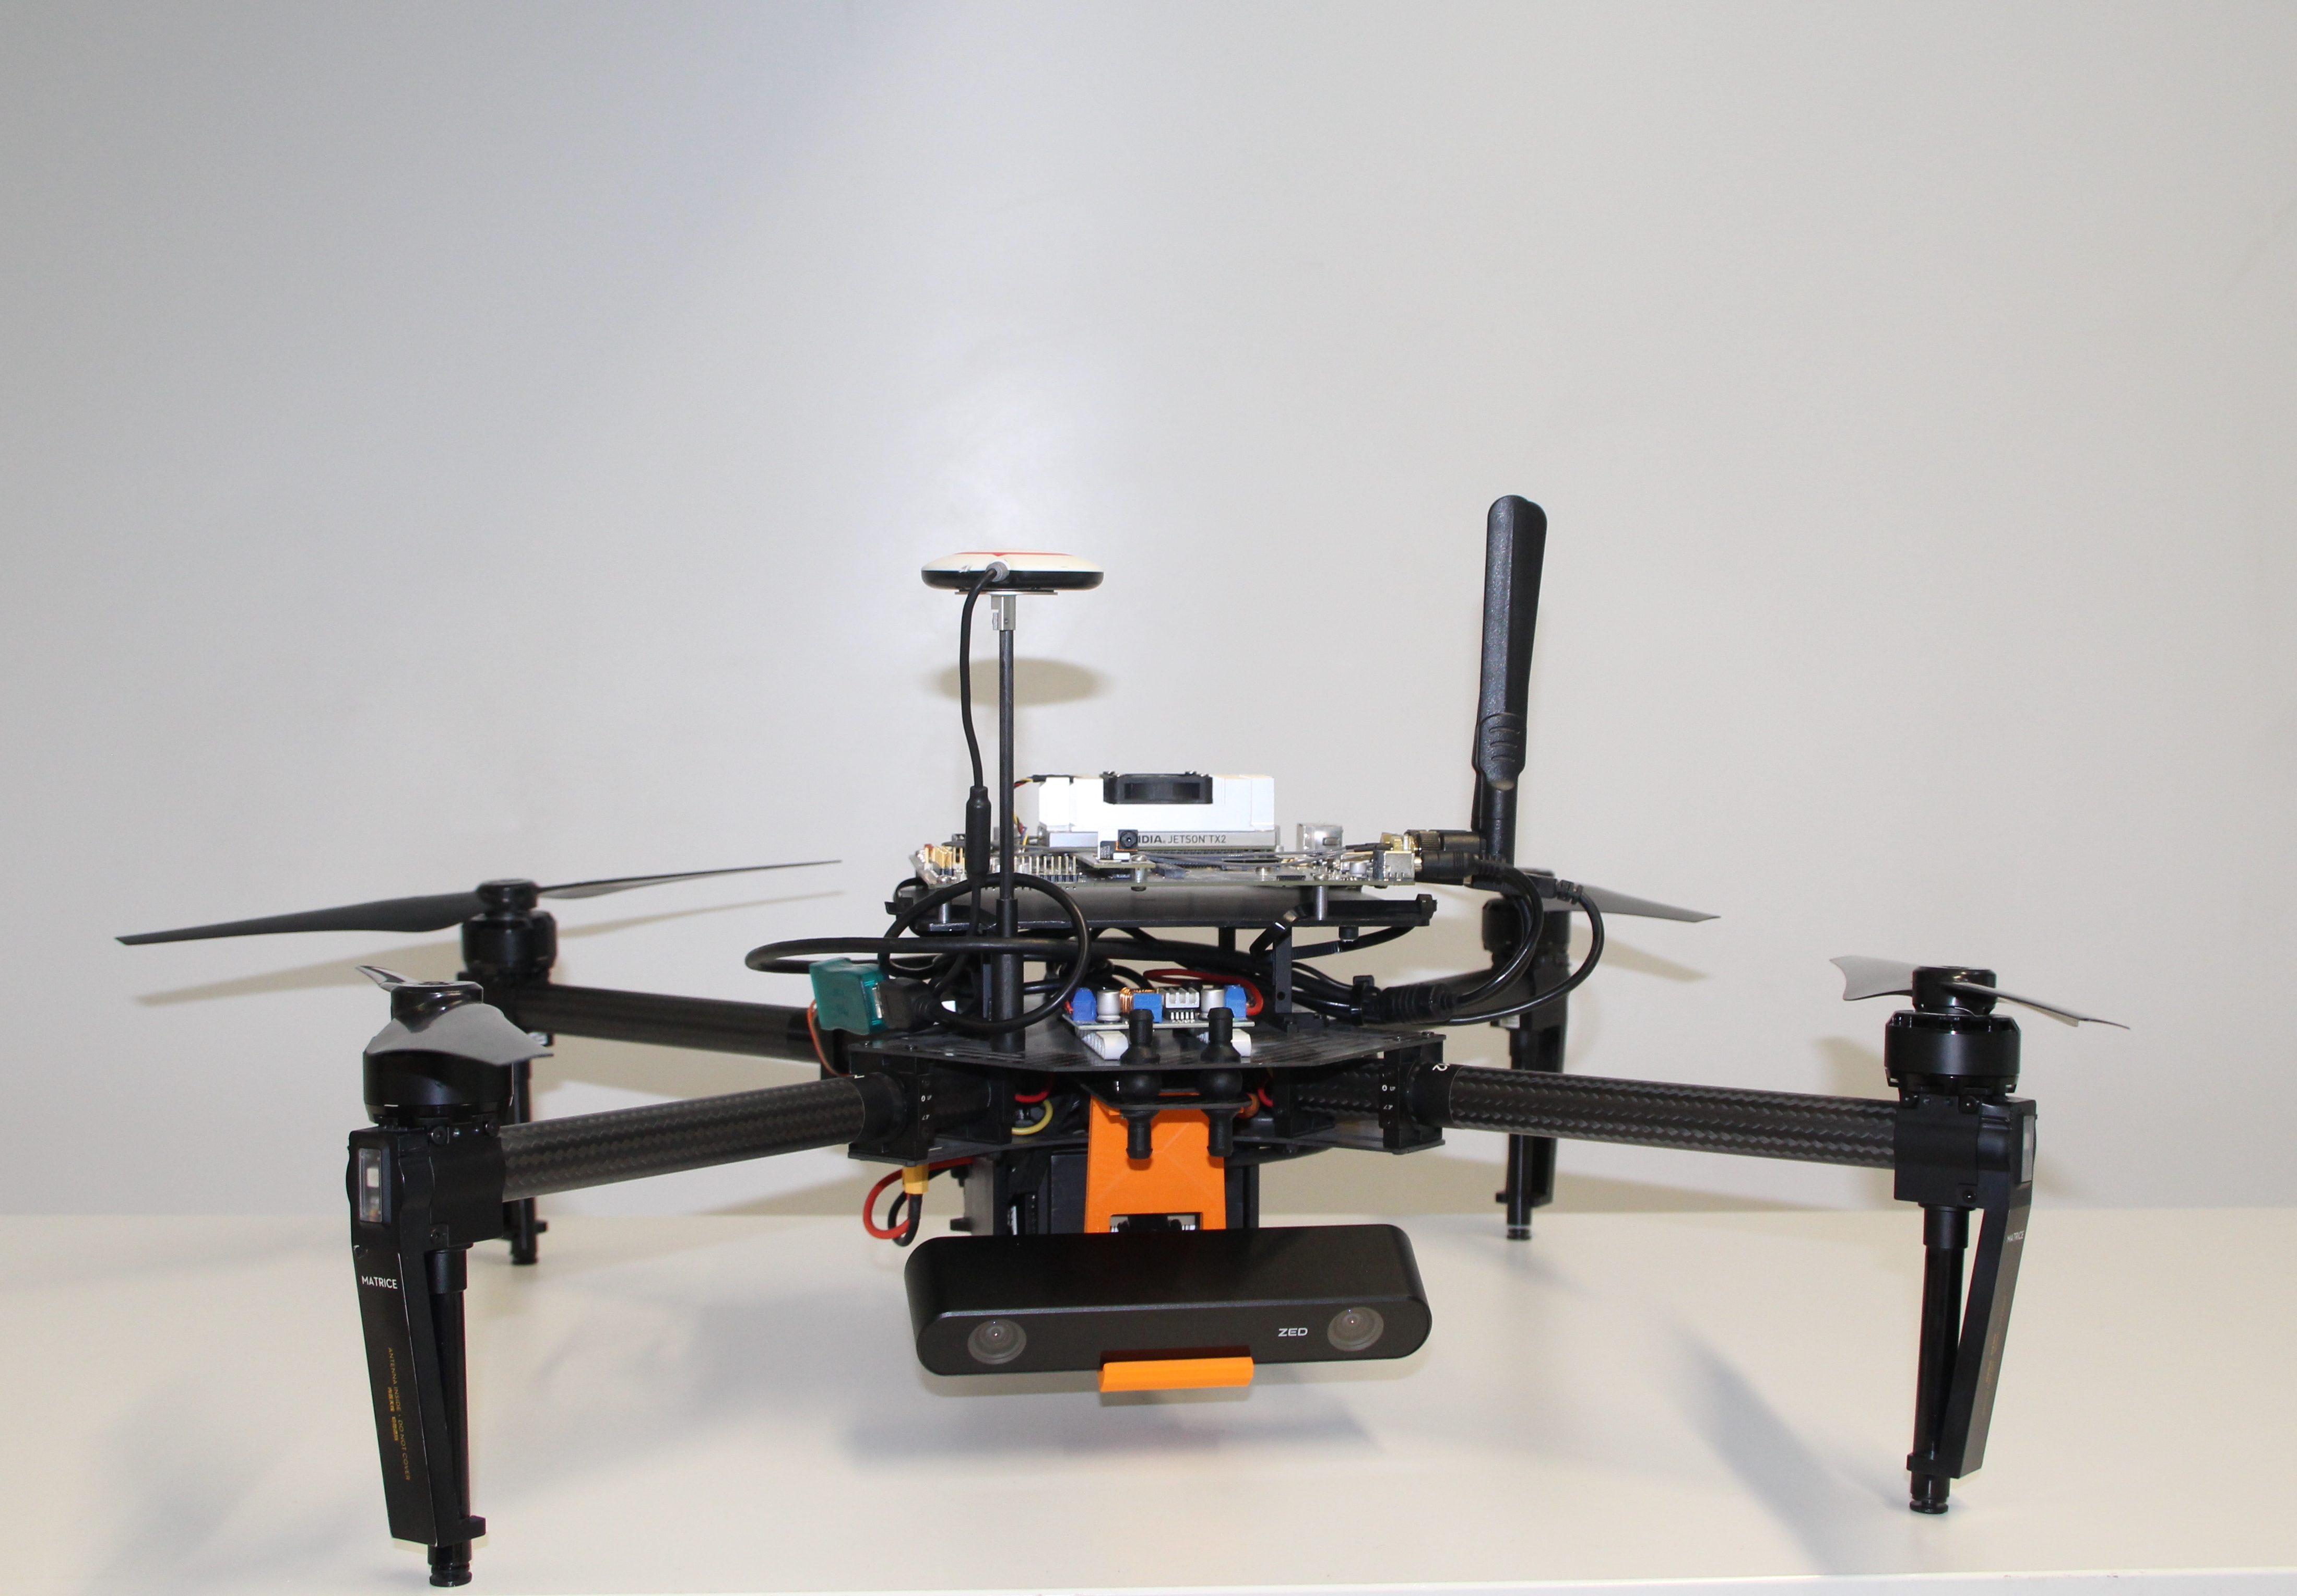
\includegraphics[width=0.9\linewidth]{img/autumnDrone}
	\caption{
		The Autumn drone with the NVIDIA Jetson TX2 on top as well as the Stereolabs ZED 2i mounted onto the drones Gimbal mounting plate using a custom 3D printed frame. 
	}
	\label{fig:autumn}
\end{figure}


\section{Autumn Lifecycle}
\textbf{Author: Fabian Kleinrad} 


\filbreak
	\chapter{Robot Operating System}
\label{chapter:ros}

\textbf{Author: Lukas Leskovar} 

This chapters objective is to describe the basic concepts of the Robot Operating System (ROS) utilized by Autumn. The ROS despite its name is a meta-operating system or middleware providing the utility and services often found in robotics frameworks. It enables the composition of distributed systems by utilizing publisher-subscriber communication between different programs of such systems. Furthermore ROS provides a comprehensive set of tools enabling the compilation, operation as well as testing, visualization and debugging of robotic systems. With its vast amount of libraries and huge open-source community providing useful functionality ROS facilitates the development of robotic applications without having to reimplement standardized technology. \footcite{openSourceRoboticsFoundationDefinitionNodate}


\section{Conceptual Overview}
The Robot Operating System can be divided into three conceptual levels each contributing a integral part to the utility of ROS. These different levels are described in the following sections. \footcite{openSourceRoboticsFoundationConceptsNodate}

\subsubsection{File System}
The File System Level mainly provides constraints and best practices for creating and structuring packages and their components. 
ROS provides appropriate tools to facilitate file-system operations with and within packages.
%operations such as searching for packages or file within packages
%With appropriate tooling the ROS facilitates file-system operations within packages, messages or topics. 

\subsubsection{Computational Graph}
The Computational Graph provides crucial functionality to ROS as it refers to the peer-to-peer mesh network of processes (nodes) each providing data to be utilized within the graph by publishing and subscribing to topics.
The concepts and technologies powering the computational graph are described in later in this chapter.

\subsubsection{Community}
The Community preserves the usability of ROS as new and useful packages and tools are created as well as existing functionality is being maintained.

\section{Naming}
To aid the organization of programs, processes as well as resources ROS provides two naming schemes that are described in the following sections. \citereset\footcite{openSourceRoboticsFoundationConceptsNodate}

\subsubsection{Graph Resource Names}
Graph Resource Names utilize a hierarchical structure to organize nodes, services, topics or anything else within the computational graph. ROS defines four different types of names:
%\begin{itemize}
%	\item base names - Are resolved in the same fashion as relative names
%	\item relative names - Are resolved relatively starting by the nodes name
%	\item global names - Begin with a / and are considered fully resolved
%	\item private names - Begin with a $\tilde{ }$ and convert the nodes name into a namespace
%\end{itemize}

\subsubsection{Package Resource Names}
Package Resource Names aim to facilitate the search process of resources at File System Level. These names usually consist of the packages name as well as the path to the desired resource within the package. 
%Examples for such Names are:
%\begin{itemize}
%	\item 
%\end{itemize}

\section{Packages}
Software in ROS is organized in packages containing nodes, libraries or any other piece of software providing functionality.

%noch ein bisschen trennen (atomic build item, ...)
%der absatz gefällt mir nicht, eigentlich gehört da nur die atomicity hin
%In order to maintain reusability, atomicity and easy decoupling of functionality packages aim to be as slim as possible by implementing only a limited-set of features. This means that each package is develop to focus on one task alone and work together with other packages to deliver utility as a connected system.
Since packages are the atomic unit of build and release they aim to be a slim as possible my implementing only a limited set of features. 
In other words packages should be implemented to provide minimal usability without being too large-scaled.\footcite{openSourceRoboticsFoundationPackageNodate} This means that each package is developed to work together with other packages to deliver utility as a connected system.  

At file-system level packages simply refer to directories. While most subfolders and files within a package depend on its purpose, every package has to contain a package.xml and a CMakeLists.txt providing meta and build information.
Packages can be build by utilizing rosbuild or catkin. \footcite{openSourceRoboticsFoundationBuildNodate}

\subsubsection{Metapackages} 
Metapackages are specialized packages only containing a package.xml that logically links multiple related packages.\footcite{openSourceRoboticsFoundationMetapackageNodate}
They can be used to conveniently install a group of packages simultaneously. %naja ned so wirklich



\section{Nodes}
The goal of ROS is to promote code reusability and decoupling of functionality to aid the versatility and usability of the system. 
Following this guideline every robotic system utilizing ROS consists of a fine-grained graph of processes called nodes. Each node provides computation on a single feature utilizing a ROS client library to communicate with others over a mesh-like peer-to-peer network. \footcite{openSourceRoboticsFoundationNodesNodate}

Exemplary for such as system would be one node running a LiDAR sensor, one responsible for localization, one performing motion planning, one controlling motor drivers and motors as well as one node running the robots main control loop.

This architecture allows for a much more fault safe and less complex applications in comparison to monolithic systems. \footcite[Page 94]{stephensBeginning2015}
This means that development and debugging are facilitated since errors can be contained within a singular slim node rather than a larger program. 

Each node has a node type consisting of the package name it is located and as well as the nodes executable. 



\section{Communication}

\subsection{Messages}
Messages are the medium of communication used in topics or services to transport data between nodes. 
%They are used to send data between nodes over topics or through services. 

\subsubsection{Message Description}
A message is a simple data structure consisting of multiple type fields. These fields can be primitives, arrays, custom types as well as other message types. \footcite{openSourceRoboticsFoundationMessagesNodate}

The message description language can be used to structure custom messages in
\textit{.msg} files contained in the \textit{msg} directory of a package.

\subsubsection{Message Types}
Message types refer to package resource names consisting of the packages name as well as the name of the messages \textit{.msg} file.


\subsection{Topics}
The core component of communication in ROS are topics. They are unidirectional message streams enabling data transmission by utilizing the publisher-subscriber model 
 %utilizing the publisher-subscriber model to establish data transmission in a many-to-many relationship.
Furthermore the decoupling of functionality is facilitated by anonymously connecting nodes as producer and consumer of data. This means neither publisher nor subscriber of the topic need to know each other. 
While ROS does not limit the amount of publishers and subscribers connected to a topic, it strictly enforces the usage of the exact message type specified for the topics communication to work properly.

\subsection{Services}
The communication architecture in ROS utilizing the publisher-subscriber model is advantageous in most use-cases, however most distributed systems require remote procedure calls (RPC) which are not supported by default.

With RPCs a client sends a request to a server specifying the procedure to be called and its parameters. While the server executes the procedure the client awaits a reply. Once the procedures results are computed and sent to the client its workflow can be resumed.\footcite[Page 3]{rfc1831}

Services enable communication over RPC by defining a pair of messages, one for requests and one for replies. Such service can then be attached to a node and called by a client using the service name. \footcite{openSourceRoboticsFoundationServicesNodate}




\section{Master}
One of the most important components of ROS is the Master. It tracks publishers and subscribers of topics as well as services and provides registration as well as name resolution to nodes. This means whenever a node wants to publish or subscribe to a specific topic or service it contacts the master first using XML-RPC. When a topic has at leat one subscriber and publisher the Master negotiates between the nodes so a peer-to-peer connection can be established using a Slave API provided by the nodes XML-RPC Server.\footcite{openSourceRoboticsFoundationMasterNodate} A simplified version of this procedure can be seen in Fig. \ref{fig:ros_master_reg}

Besides registration and name resolution, the ROS Master also provides a Parameter Server used for globally storing static system parameters.\footcite{openSourceRoboticsFoundationParameterServerNodate}
\begin{figure}[]
	\centering
	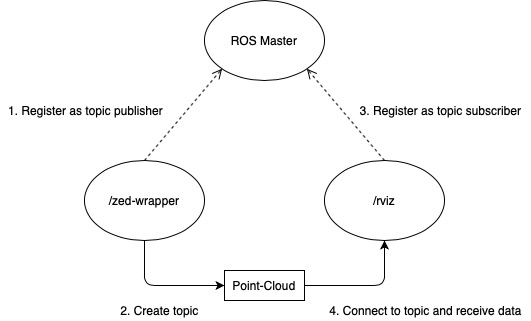
\includegraphics[width=0.8\linewidth]{img/ros_master_registration}
	\caption{Diagram of the topic registration process in ROS at which the publishing node registers its topic before the subscriber tells the master its interest in the point-cloud topic. However a node can be registered as a subscriber to a specific topic without the topic existing yet.}
		\label{fig:ros_master_reg}
\end{figure}



\section{Transform Library}
A complex robotic system consists of multiple parts such as sensors, cameras, manipulators, etc. which are each represented as a coordinate frame, where each frame is connected to another frame using joints. When trying to move a specific part or coordinate frame, not only the transform of that single frame but the composite transform of each frame in relation to the target has to be calculated. This is especially important when moving a robotic arm based on sensor readings. In this example a transform between the position of the sensor and the arm needs to be calculated so the motion performed by the arm the motion perceived by the sensor match.
Using the ROS Transform Library (tf) these complex calculations can be facilitated. To this end tf keeps track of each coordinate frame in a acyclic relationship tree where tf broadcasters then publish relative pose information and listeners query transforms between two coordinate frames. 
Because not all pose information in a robotic system is instantly accessible, the tf saves this information for each frame over time. This means that transforms can be queried not just spacially but also temporally.



\section{Simulation}
Debugging and testing robot applications can be a repetitive and tedious task, especially when a test environment needs to be reset at every test cycle. In order to facilitate this part of development the Autumn robot utilises the representation and simulation technologies that are described in the following sections.

\subsection{URDF}
In order to perform simulations or compute coordinate frame transforms a robot needs to be described in some way. One of the more popular description formats is the Unified Robot Description Format (URDF) which provides a XML format for representing a robot and its components as well as a \textit{C++} parser and tools to convert and verify and visualize these models. \footcite{openSourceRoboticsFoundationURDFNodate}
The \textit{check\_urdf} tool parses a URDF-File and returns the robots kinematic chain if successful.
To visualize the robots frames and joints in a graphviz\footcite{graphvizAuthorsAboutNodate} tree the \textit{urdf\_to\_graphiz} tool can be used. The resulting tree corresponds to the relationship tree tf uses to calculate transforms.

\subsection{Gazebo Simulator}\label{section:gazebo}
Gazebo is a 3D physics simulator often used in close relation to ROS projects. Therefore it provides tooling for model and world design and generation as well as comprehensive interfaces for controlling a simulated robot through ROS. Further advantages of Gazebo are its accurate sensor and sensor noise generation as well as its large community providing countless models of robots and sensors. \footcite{openSourceRoboticsFoundationGazeboNodate}
%vielleicht noch über URDF SDF schreiben - aber erst wenn simulation von autumn fertig ist

\filbreak
	\chapter{Sensors and measurements}

\textbf{Author: Lukas Leskovar} 

The means of perceiving ones surrounding environment are a crucial part of any robotic system. This chapter aims to describe the need for interoceptive measurements aiding the different algorithms used within Autumn as well as any sensory equipment supporting such data acquisition. To this end the underlying principles and concepts behind the measurement techniques and  are illustrated.

\section{Motion Models}
Kinematic models in robotics are used for describing and planning state-transitions between consecutive robot poses. While Chapter \ref{chapter:slam} focuses on the theoretic basics of such models and how to build upon them, this section is going to focus on the practical concepts used in robot localization. To this end classical odometry as well as velocity based motion models are described.
To facilitate any equations later in this section the robot pose is described by its state vector 
\[
\begin{pmatrix}
	x \\
	y \\
	\theta \\
\end{pmatrix}
\] 
which defines its position as Cartesian coordinates and bearing as angular orientation $\theta$ in 2 dimensional space. 

\subsection{Odometry}
Ben-Ari and Mondada define this topic as follows: "Odometry—the measurement of distance—is a fundamental method used by robots for navigation.". \footcite[Page 69]{ben2017elements} 
When performing linear odometry, e.g. without taking orientation changes into consideration, this distance is calculated rather trivially by inferring it through measured time elapsed and the velocity of the robot proportionally to the motor power. 
Other systems however utilize wheel encoders to count the number of wheel rotations thus allowing for rather precise estimation of distance. 

With non-linear motion the distances $d_{l}$ and $d_{r}$ moved by the left and right wheel are unequal which requires the calculation of both updated position and bearing of the robot. 
Lets suppose a robot moved from position $\begin{pmatrix} x & y & \theta \end{pmatrix}^{T}$ to $\begin{pmatrix} x' & y' & \theta' \end{pmatrix}^{T}$ with a slight left turn caused by the right wheel turning faster than the left one. 
This scenario is depicted in Fig. \ref{fig:odom} with $\varphi$ corresponding to the turn angle in radians, the radii $r_{l}, r_{c}, r_{r}$ describing the distance from the new position of the wheels and center to point $P$, the origin of the turn. 

For small angles these radii are approximately the same length as the distances $d_{l}, d_{c}$ and $d_{r}$, which allows for the turn angle to be calculated as follows:
\begin{align*}
	\varphi &= \frac{d_{i}}{r_{i}}, & i &= l, r, c  
\end{align*}

However in practical scenarios where these radii and the point P are unknown, $\varphi$ has to be calculated only using $d_{l}$, $d_{r}$ and $b$ which corresponds to the distance between both robot wheels.

\begin{equation*}
	\begin{split}
		\varphi r_{r} = d_{r} \\
		\varphi r_{l} = d_{l} \\
		\varphi r_{r} - \varphi r_{l} = d_{r} - d_{l} \\
		\varphi = \frac{d_{r} - d_{l}}{r_{r} - r_{l}} \\ 
		\varphi = \frac{d_{r} - d_{l}}{b} \\
	\end{split}
\end{equation*}

To calculate the new coordinate positions the distance $d_{c}$ is computed:
\begin{equation*}
	d_{c} = \frac{d_{l} + d_{r}}{2}
\end{equation*}

The final pose is calculated as follows:

\begin{equation*}
	\begin{pmatrix}
		x' \\ 
		y' \\
		\theta'
	\end{pmatrix}
	= 
	\begin{pmatrix}
		-d_{c} \sin \varphi \\
		d_{c} \cos \varphi \\ 
		\theta + \varphi
	\end{pmatrix}
\end{equation*}

Because the assumptions above only apply for small distances in any real-world systems such computations ought to be performed continuously. However due to uncertain measurements these calculations inherit some margin of error which is integrated up over multiple iterations thus causing a slight drift in the output.\footcite[Pages 69 - 77]{ben2017elements} 
This drift can be corrected using techniques discussed in Chapter \ref{chapter:slam}.

\begin{figure}
	\centering
	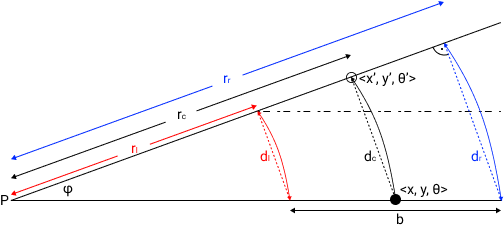
\includegraphics[width=0.8\linewidth]{img/odom}
	\caption{
		This diagram shows the geometry of how a slight turning motion can be calculated only using the distances $d_{l}$, $d_{r}$ and wheel offset $b$.
		The robot pose 
		$
			\begin{pmatrix}
				x &
				y &
				\theta 
			\end{pmatrix}^{T}
		$
		is associated with the center of the robot.
	}
	\label{fig:odom}
\end{figure}


\subsection{Inertial Measurement}
Another way of modelling motion usually utilized when a robot is not equipped with wheel encoder nor wheels is based on velocities influencing the vehicle. Typically the inputs of velocity based motion models are measured used Inertial Measurement Units (IMU), Gyroscopes and Accelerometers. 

These velocities $v$ and $\omega$ as the translational, linear and angular velocity are referred to as controls for the system. 
In contrast to odometry which can only be calculated after a movement has been performed these controls allow for prior motion planning. \footcite[Pages 92 - 99]{thrun2002probabilisticRobotics}

If these velocities stay fixed for the entire duration $\Delta t$ of the motion from 
$\begin{pmatrix} x & y & \theta \end{pmatrix}^{T}$
to
$\begin{pmatrix} x' & y' & \theta' \end{pmatrix}^{T}$
the robot moves in a circle with radius $r$ as seen in Fig. \ref{fig:inertial}. The center $P$ of this circle with coordinates 
$
\begin{pmatrix}
	x_{P} & y_{P}
\end{pmatrix}
^{T}
$
can be evaluated as follows:

\begin{equation}
	\begin{split}
		x_{P} = x - \frac{v}{\omega} \sin \theta \\
		y_{P} = y + \frac{v}{\omega} \cos \theta
	\end{split}
\end{equation}

This allows for the new position to be calculated: 

\begin{equation}
	\begin{pmatrix}
		x' \\
		y' \\
		\theta'
	\end{pmatrix}
	=
	\begin{pmatrix}
		x_{P} + \frac{v}{\omega} \sin(\theta + \omega \Delta t) \\
		y_{P} - \frac{v}{\omega} \cos(\theta + \omega \Delta t) \\
		\theta + \omega \Delta t
	\end{pmatrix}
\end{equation}

Despite incapable of calculating movements in advance, odometry ought to be preferred over velocity motion models as they pose higher accuracy in localization. \footcite[Page 107]{thrun2002probabilisticRobotics}

\begin{figure}
	\centering
	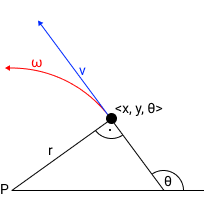
\includegraphics[width=0.5\linewidth]{img/inertial}
	\caption{
		In this diagram a slight turning motion of the robot is described by the translational velocity $v$ and angular velocity $\omega$. These velocities if consistent render the robot to move in a perfect circle with center $P$ and radius $r = | \frac{v}{\omega}|$. Even if the angular velocity remains 0 the motion is still described as a circle with an infinite radius.
	}
	\label{fig:inertial}
\end{figure}



\section{Depth Sensing}
Similar to motion models contributing to robot localization in Autumn, Depth Sensing is utilized to perceive and map the drones environment. 
The technologies in this section focus on mapping distance information to each point in the cameras field of view thus providing 3D-Imaging.

\subsection{Structured Light}
One approach uses active illumination to project a varying intensity pattern onto the perceived scene thus allowing for a camera to extract 3D-information from the distorted pattern as the surface of the scene is non-planar. \footcite{geng2011StructuredLight}

\subsection{Time-of-Flight}
Time-of-Flight (ToF) sensors perform active triangulation, which is performed by emitting a modulated ray of light which is reflected by the scene, as described in Fig. \ref{fig:activeTriangulation}. The distance to the scene is determined using the time difference between emition and detection (more prominent with ToF Laser-Scanners like LiDAR) or the phase shift of the waves reflected by the whole scene. The latter allows for mapping depth information to the entire Field-of-View (FoV) of the sensor or camera. 
%It may be necessary to differentiate mapping using depth perception sensors from LiDAR technologies which pose an alternative solution. 
Although LiDAR sensors fall under the category of ToF sensors they perceive the distance to an object using pulsed lasers thus outputting
the distance to singular points in the sensors environment rather than depth information mapped to an image. \footcite{gokturk2004time} \footcite{velodyne2021LiDAR}
% LiDAR verwenden die Zeitdifferenz und berechnen mittels Trigonometrie die Distanz
As 3D-LiDAR sensors applied in many commercial mapping solution are very expensive they disqualify for use in Autumn as it focuses on performing with approximate precision using relatively inexpensive camera based equipment. 

\begin{figure}
	\centering
	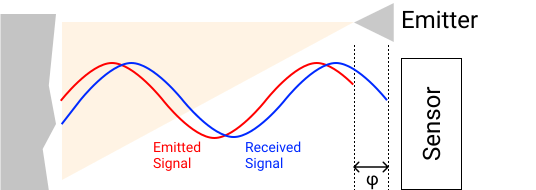
\includegraphics[width=0.8\linewidth]{img/activeTriangulation}
	\caption{
		This diagram depicts how a ToF sensor utilizes the phase-shift $\varphi$ between the emitted IR-Light (red) and received signal (blue). 
		% noch mehr schreiben
	}
	\label{fig:activeTriangulatoin}
\end{figure}


\subsection{Stereo Vision}
The last and most significant approach to Autumn performs passive triangulation using two cameras setup as seen in Fig. \ref{fig:passiveTriangulation}. Although this eliminates the need for any light to be emitted however the problem of correspondence is introduced, which deals with associating the different projections to the same point in the real world. There are multiple approaches to this problem which are generally divided into global and local matching methods with the latter being more computationally efficient while sacrificing quality.\footcite{do2019review}

In Autumn this approach was pursued using a Stereolabs ZED depth camera as it was superior to any competitors such as the Microsoft Kinect or Intel Realsense concerning availability and cost-effectiveness. 

\begin{figure}
	\centering
	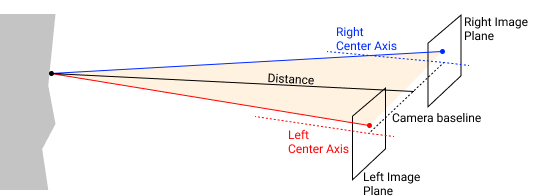
\includegraphics[width=0.8\linewidth]{img/PassiveTriangulation}
	\caption{
		This diagram describes the camera setup found in passive triangulation systems. Using stereo-photogrammetry the distance to the perceived scene is calculated. 
	}
	\label{fig:passiveTriangulation}
\end{figure}

\subsection{ZED 1 vs ZED 2}
%As mentioned in Chapter \ref{chapter:architecture} the Stereolabs ZED 1 was used in a first prototype and later replaced with a 
Chapter \ref{chapter:architecture} mentions that the Stereolabs ZED 1 used in early prototypes was quickly replaced with the ZED 2. This change was due to processing limitations and additional features provided by the newer product version.
This section aims to benchmark the two cameras from a depth-performance standpoint to review if the upgrade enhanced depth perception thus improving the system output or if no changes were necessary when only considering depth-perception.

\subsubsection{Experiment}
To answer this question the cameras measured the vertical distance enclosed by two points mounted $1m$ above each other on a stationary structure with the bottom one at a height $1m$ above the ground. 
The cameras was paced on a movable rig normal to the stationary structure and 1m above the ground.  The aforementioned gap was measured by the cameras at $1m$ increments between $3m$ and $10m$ horizontal distance measured amongst each structures base. 

The usage of ARUCO markers allowed for precisely tracking the position of each point within the camera coordinate system thus ensuring the points remain fixed even though the camera rig is moved. 
% über ARUCO schreiben
% reference zu ARUCO 
ARUCO markers are squared-based markers popular in many robotic and augmented reality applications as they provide a fast and robust solution for estimating a cameras pose. Each marker has a unique, identifiable pattern which allows for precisely determining and tracking its position.\footcite{jurado2015} 

\subsubsection{Results}
%Fig. \ref{plot:zedBenchmark} depicts the mean depth-perception error measured thus indicating how well each camera performed. 

The mean depth-perception error dependant on the camera distance for the ZED 1 (blue) is plotted in Fig. \ref{plot:zedBenchmark}. To illustrate the positive tendency a linear regression (cyan) is superimposed. The trend line indicates a relatively steep slope with the mean error adding up by $0.03m$ at increasing distances from the rig. Additionally the error range listed in Tab. \ref{tab:errorMinimaMaxima} shows a base error of 0.7\% and a maximum mean error of 3\%, which is similar to the error stated by the cameras data sheet\footcite{zed1Datasheet}.

The data for the ZED 2 (red) and its corresponding trend line (orange) indicate a much more shallow slope with $0.01m$ per meter distance to the rig. Looking at the error range the ZED 2 lies below 1\% mean error at all distances which also corresponds to the data sheets specifications \footcite{zed2Datasheet}.


%When comparing each trend line for each camera it is apparent that the slope of the ZED 1 with $0.03m/m$ is more than twice as large compared to the ZED 2 at $0.01m/m$. This indicates that with increasing distance the depth-perception error increases dramatically. 
%Another interesting finding are the minima and maxima of the mean depth-perception error found in Tab. \ref{tab:errorMinimaMaxima}.
%As illustrated the ZED 1 inherits a substantially large minimal and maximal error of  $0.07m$ and $0.31m$.
%Compared to this the ZED 2 performed much better with a almost non existent base error and a maximal error of $0.1m$.

\begin{table}[h]
	\centering
	\begin{tabular}{|l|l|l|}
		\hline
		& \textbf{Minimal Mean Error} & \textbf{Maximal Mean Error} \\ \hline
		\textbf{ZED 1}  & 0.07m 					  & 0.31m                      \\ \hline
		\textbf{ZED 2} & 0.01m                      & 0.10m                      \\ \hline
	\end{tabular}
	\caption{Table containing the minimal and maximal mean error of both the ZED 1 and ZED 2.}
	\label{tab:errorMinimaMaxima}
\end{table}

\begin{figure}[h]
	\begin{center}
		\begin{tikzpicture}
			\begin{axis}[
				width=0.8\linewidth, % Scale the plot to \linewidth
				grid=major, 
				grid style={dashed,gray!30},
				xlabel={Distance [m]}, % Set the labels
				ylabel={Mean Error [m]},
				legend pos=north west,
				xtick={3, 4, 5, 6, 7, 8, 9, 10},
				xmin=2,
				xmax=11,
				ymin=0,
				ymax=0.35,
				]
				
				
				%zed1 data
				\addplot[only marks, color=blue]
				table[row sep=crcr]{
					distance error \\
					0 0 \\
					3 0.072842 \\
					4 0.084444 \\
					5 0.090908 \\
					6 0.082350515 \\
					7 0.091252505 \\
					8 0.136357778 \\
					9 0.170380567 \\
					10 0.306662651 \\
				}; 
				\addlegendentry{ZED1}
				
				%zed1 regression
				\addplot[no marks, color=cyan, style=dashed]
				table[row sep=crcr, y={create col/linear regression={y=error}}]{
					distance error \\
					0 0 \\
					3 0.072842 \\
					4 0.084444 \\
					5 0.090908 \\
					6 0.082350515 \\
					7 0.091252505 \\
					8 0.136357778 \\
					9 0.170380567 \\
					10 0.306662651 \\
				};
				\addlegendentry{$y = 0.03x + 0.04; R^2 =  0.67$} 
				
				%zed2 data
				\addplot[only marks, color=red]
				table[row sep=crcr]{
					distance error \\
					0 0 \\
					3 0.005048 \\
					4 0.010964 \\
					5 0.058536585 \\
					6 0.080308 \\
					7 0.045865731 \\
					8 0.040048 \\
					9 0.102566462 \\
					10 0.081332636 \\
				}; 
				\addlegendentry{ZED2}
				
				%zed2 regression
				\addplot[no marks, color=orange, style=dashed]
				table[row sep=crcr, y={create col/linear regression={y=error}}]{
					distance error \\
					0 0 \\
					3 0.005048 \\
					4 0.010964 \\
					5 0.058536585 \\
					6 0.080308 \\
					7 0.045865731 \\
					8 0.040048 \\
					9 0.102566462 \\
					10 0.081332636 \\
				}; 
				\addlegendentry{$y = 0.01x + 0.02; R^2 =  0.58$}
			\end{axis}
		\end{tikzpicture}
		\caption{This plot describes how the mean depth-performance error of both the ZED 1 (blue) and ZED 2 (red) Stereo Camera changes with increasing distance to an object. Furthermore the linear regression function for both the ZED 1 (cyan) and ZED 2 (orange) are plotted. 
		 }
	 	\label{plot:zedBenchmark}
	\end{center}
\end{figure}


Comparing both trend lines and mean error range the ZED 1 clearly shows a much more aggressive upwards trend and higher base error compared to the ZED 2. However as the coefficient of determination $R^{2}$ for each trend line indicate a mediocre fit the aforementioned assumptions should not be solely taken into consideration when comparing the two camera systems. 
Having said this, in combination with the data sheets, the overall trend on depth-performance meets the initial assumption and justifies the upgrade to the ZED 2.

%Considering all of the aforementioned findings it is apparent that the ZED 2 produced much better depth-perception results compared to the ZED 1. This justifies the upgrade not only from a feature focused standpoint but also quality wise as this greatly effects the final 3D point cloud utilized by components discussed later in this thesis. 

\filbreak
	\chapter{Simultaneous Localization and Mapping}
\label{chapter:slam}

\textbf{Author: Lukas Leskovar} 

%frame of reference klingt nicht so gut
The problem of localizing as well as navigating a system through a completely or partly unknown environment without any external coordinate system (i.e. GPS, Optical Beacon Tracking, etc.) has proven itself to be one of the most complex and yet fundamental topics in many scientific research fields with robotics being most prominent. The main approach to this problem is Simultaneous Localization and Mapping (SLAM) which dates back to the mid 1980s. Back then the first solutions based on Extended Kalman Filters or Rao-Blackwellised Filters were formulated. \footcite{durrantSlam2006}  \footcite{cadenaSlamFuture2016}

To date the topic of SLAM has matured, algorithms have gotten more reliable and robust and are utilized in many industries. Applications for SLAM range from navigating a Mars-Rover over autonomous cars or warehouse robots to simple household appliances like vacuum cleaners. 

As one major topic of this thesis is robot navigation in a GPS-denied area as well as mapping of such environment, different modern SLAM approaches and solutions utilized by the project team are discussed in this chapter.

\section{Localization}
%state estimation beschreiben dass pose sowie andere informationen wie geschw. usw. erfasst werden. 
Localization or state-estimation aims to reconstruct the state of a system using interoceptive measurements (e.g. acceleration, velocity, etc.) as well as an exteroceptive model (e.g. position and orientation) of the system. \footcite[Pages 3 - 5]{barfootStateEstimation2017}
Put into the context of mobile robotics this means that in order to perform comprehensive localization of a mobile robot a sensor fusion between on-board sensors and a global coordinate system ought to be performed as solely relying on sensor data such as odometry would quickly result in large accumulated errors.
%Exemplary for such a robot would be a drone utilizing a Inertial Measurement Units (IMU) odometry as well as GPS positional data to estimate its current position.
An exemplary system for this would be an industrial robot utilizing a construction plan to correct errors by wheel-encoded odometry to navigate through a factory. 

\section{Mapping}
Contrary to localization, in mapping problems the current pose of the system is known while its environment remains uncharted.
Therefore stand-alone mapping aims to generate a model of its environment by evaluating sensor readings of environmental features as well as the systems pose to reconstruct aforementioned features in a global reference frame. 
Mapping applications often combine technologies typically found in other scientific fields such as photogrammetry or computer vision.
An example for such a system would be a drone computing camera images and GPS positional data with a photogrammetric algorithm to reconstruct a 3D-Model of a building. 


\section{Localization and Mapping}
The aforementioned technologies on their own are considered rather simplistic problems as either the environments map is given or a reliable pose-estimation can be provided. While most applications meet either of these criteria with pre-built maps or GPS being available, some environments such as buildings, mineshafts or outer space both the systems pose and environment remain uncertain and need to be determined simultaneously hence the name Simultaneous Localization and Mapping. 
To summarize, the crux of the SLAM problem, as described in Fig. \ref{fig:slamOverview}, is that localizations requires a map and mapping depends on pose estimates however neither are certain. 

%The following sections will mainly focus on the SLAM back-end and dissect the problem by reviewing different probabilistic approaches. 


%In order to partially solve this dilemma SLAM incorporates loop closure to correct the global map as well as positional estimates provided by odometry. A loop closure event occurs when revisiting previously mapped landmarks and associating relations between features to adapt the global topology. %Without loop closure a mobile robot would perceive its environment as a infinite corridor.


\begin{figure}
	\centering
	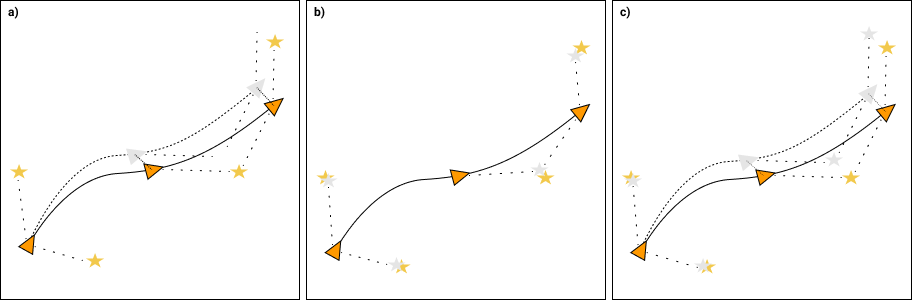
\includegraphics[width=1.0\linewidth]{img/slamOverview}
	\caption{
		The figure above depicts the different tasks contributing to the SLAM problem. Panel a) shows a robot (triangles) moving trough a known environment while the pose and path remain uncertain. In panel b) the robots pose is certain while the landmark (stars) locations need to be determined. Panel c) composes both previous problems where neither the robot state nor the landmark locations are certain. \footcite{durrantSlam2006}
	}
	\label{fig:slamOverview}
\end{figure}

\section{Map Representation}
The way a robot perceives its surroundings and maintains a accurate map is directly dependant on many criteria such as complexity of tasks, size of its environment as well as measurement quality mainly influenced by sensor noise. 
Tailoring to benefit some of the aforementioned criteria most robotic mapping systems utilize either of two paradigms, metric or topological, each proposing their respective strengths and weaknesses.

Metric or grid-based maps build a map of the robots environment as occupancy grids, with each cell indicating the presence of an obstacle. The main benefit using metric maps is the facilitated construction of large-scale mappings as well as non-ambiguous determination of places. However such maps have significant drawbacks concerning space as well as time complexity and require accurate pose estimation of the robot.

Topological or feature-based maps reconstruct their environment as graphs with each node representing a feature or landmark perceived by the robots sensors. In contrast to metric maps they allow for comprehensive path planning and are significantly more compact as its resolution is directly proportional to the environments complexity. \footcite{thrunMaps1998}


\section{Probabilistic Definition}
To describe probabilistic SLAM lets assume a robot is moving through an environment observing multiple landmarks at different times. 
The goal is that, for any time instant $ t $, the robots state vector 
\[ x_{t} = 
\begin{pmatrix}
	x \\
	y \\
	\theta \\
\end{pmatrix}
\] as well as a time invariant set of all absolute landmark positions 
% describing its position and orientation as well as a time invariant set of all absolute landmark positions 
% umformulieren dass es nicht heißt der state vector beschreibt die landmarks
$ m = \{ m_{1}, m_{2}, ..., m_{i} \}$ 
is computed, given uncertain relative landmark observations $ z_{0:t} = \{z_{0}, z_{1}, ..., z_{t}\}$, controls $ u_{0:t} = \{u_{0}, u_{1}, ..., u_{t}\}$ and known initial location $ x_{0} $. Fig. \ref{fig:slamGraphical} depicts this process and illustrates the relationships between the variables important in any SLAM system. 

\begin{equation}\label{fullSLAM}
	P(x_{0:t}, m | z_{0:t}, u_{0:t}, x_{0})
\end{equation}

In \ref{fullSLAM}, which is often referred to as "Full-SLAM" or "Offline-SLAM", the joint posterior density of the robots trajectory and landmark locations is estimated. In other words, this formulation of the problem aims to recover the whole robot trajectory.

\begin{equation}\label{onlineSLAM}
	P(x_{t}, m | z_{0:t}, u_{0:t}, x_{0})
\end{equation}

The pendant to this is "Online-SLAM" which aims estimate only the robots latest location at time instant $ t $, as seen in \ref{onlineSLAM}. In contrast to "Full-SLAM", performing batch computation on the whole data, algorithms pursuing this online approach typically compute the probability distribution incrementally. 

\begin{figure}
	\centering
	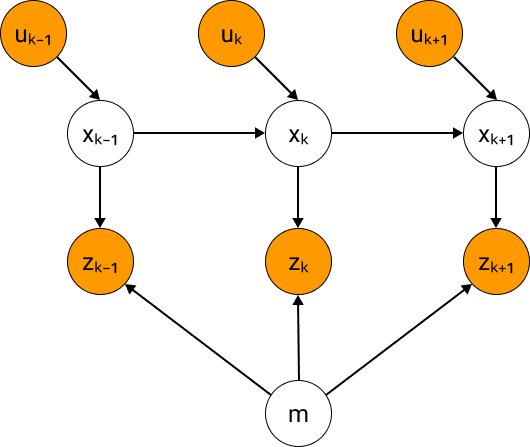
\includegraphics[width=0.4\linewidth]{img/SlamGraphical}
	\caption{
		A Bayes network graph depicting the causal relationships between sensor measurements (orange circles) and uncertain variables (white circles). It is made apparent how the relative measurements by odometry or landmark observation influence the robot state as well as landmark locations. 
	}
	\label{fig:slamGraphical}
\end{figure}

To compute either problem a mathematical model representing the robots state transition and a model describing observations ought to be defined:

\begin{equation}\label{motionModel}
	P(x_{t} | x_{t-1}, u_{t})
\end{equation}

\begin{equation}\label{observationModel}
	P(z_{t} | x_{t}, m)
\end{equation}

The motion model \ref{motionModel} describes the robots location at time $ t $ given a known previous location $ x_{t-1} $ and control $ u_{t} $ assuming the state-transition is a Markov process \footcite{haeneltMarvoModel2006}.
\ref{observationModel} calculates the probability of observing a landmark $ z_{t} $ when the robots location $ x_{t} $ and environment $ m $ are known.
\footcite{durrantSlam2006}
 %For aforementioned reasons in SLAM the map is not known to the system, therefore many formulations omit the map in the observation model.

%The joint posterior is then implemented in a recursive prediction and correction form which is often described as time-update and measurement-update:

For filtering approaches which are discussed later in this chapter, the joint posterior is then implemented in a recursive prediction and correction form which is often described as time-update and measurement-update:

\begin{equation}\label{timeUpdate}
	P(x_{t}, m | z_{0:t-1}, u_{0:t}, x_{0}) = \int P(x_{t} | x_{t-1}, u_{t}) P(x_{t-1}, m | z_{0:t-1}, u_{0:t-1}, x_{0}) dx_{t-1}
\end{equation}


\begin{equation}\label{measurementUpdate}
	P(x_{t}, m | z_{0:t}, u_{0:t}, x_{0}) = \frac{P(z_{t} | x_{t}, m) P(x_{t}, m | z_{0:t-1}, u_{0:t}, x_{0}))}{P(z_{t} | z_{0:t-1}, u_{0:t}}
\end{equation}

The time update in \ref{timeUpdate} calculates an estimate of the robots state using a previously known state at $ t - 1 $ and state-transition given the newest control $ u_{t} $.
In the next step, the measurement update \ref{measurementUpdate}, a observation $z_{t} $ is taken and the previously calculated estimate is corrected using Bayes-Theorem\footcite{durrantSlam2006}. 

To make the the recursive structure of such filtering approaches more apparent the equations \ref{timeUpdate} and \ref{measurementUpdate} can be compared to the Bayes filter algorithm, commonly used as framework for further state-estimation problems\footcite[Page 23]{thrun2002probabilisticRobotics}.

\begin{equation}\label{timeUpdateBayes}
	\overline{\rm bel}(x_{t}) = \int P(x_{t} | x_{t-1}, u_{t})  bel(x_{t-1}) dx_{t-1}
\end{equation}


\begin{equation}\label{measurementUpdateBayes}
	bel(x_{t}) = \eta  P(z_{t} | x_{t})  \overline{\rm bel}(x_{t-1})
\end{equation}

\section{Solution Paradigms} 
Over time many different approaches to the SLAM problem have been developed which can be categorized into either of three paradigms. The two mature ones are based on recursive filtering techniques while the modern graph-based solutions perform non-linear sparse optimization.

\subsection{Extended Kalman Filter}
The Extended Kalman Filter (EKF) is one of the first approaches to the Online-SLAM problem and a extension of the Kalman Filter (KF). Contrary to the standard KF it is applicable to non-linear systems by performing linear approximation.

%The Extended Kalman Filter (EKF) is one implementation of a Bayes Filter for non-linear problems and was one of the first approaches to the Online-SLAM problem. The author recommends preliminary knowledge about Bayes Filters\footcite{tipaldiBayes2020}, the vanilla Kalman Filter and the EKF\footcite{tipaldiEKF2020} before reading this section about its application in SLAM. 

The Kalman Filter assumes a environment in which landmarks can be fully represented as points within the coordinate frame. The earlier introduced state-vector $ x $ is extended to a state-space vector with dimensions $ 3 + 2n$
\[ \mu = 
\begin{pmatrix}
	x \\
	m \\
\end{pmatrix}
=
\begin{pmatrix}
	x & y & \theta & m_{1, x} & m_{1, y} & \dots & m_{n, x} & m_{n, y} 
\end{pmatrix} ^{T}
\] 
to incorporate $n$ landmark locations. 

Furthermore a covariance matrix 
$ \Sigma = 
\begin{pmatrix}
	\Sigma_{xx} & \Sigma_{xm} \\
	\Sigma_{mx} & \Sigma_{mm} \\
\end{pmatrix} $ 
is introduced which specifies the state $ x $ and landmark $ m $ uncertainties as well as correlations between landmarks and robot pose. 

The motion and observation models are implemented as non-linear functions $x_{t} = g(u_{t}, x_{t - 1}) + \epsilon_{t}$ and $z_{t} = h(x_{t}) + \delta_{t}$ with $\epsilon_{t}$ and $\delta_{t}$ defined as random noise variables.% commonly based on zero-mean additive Gaussian noise.

%defined as non-linear Gaussian distributions $ \mathcal{N}(g(u_{t}, x_{t - 1}), R_{t}) $ and $ \mathcal{N}(h(x_{t}), Q_{t}) $ based on non-linear functions $g$ and $h$ with $ R_{t} $ and $ Q_{t} $ representing zero-mean additive Gaussian noise.
To still calculate the state transition as well as measurement update these functions are linearized by performing first order Taylor Expansion\footcite[Pages 33-51]{thrun2002probabilisticRobotics}.

%\begin{equation}
%	g(u_{t}, x_{t - 1}) \approx g(u_{t}, \mu_{t - 1}) + g'(u_{t}, \mu_{t - 1})(x_{t - 1} - \mu_{t - 1}) 
%	= g(u_{t}, \mu_{t - 1}) + G_{t}(x_{t - 1} - \mu_{t - 1})
%\end{equation}
%
%\begin{equation}
%	h(x_{t}) \approx h(\overline{\mu}_{t}) + h'(\overline{\mu}_{t})(x_{t} - \overline{\mu}_{t}) 
%	= h(\overline{\mu}_{t}) + H_{t}(x_{t} - \overline{\mu}_{t})
%\end{equation}

This allows for the functions to be incorporated in the vanilla Kalman Filter Algorithm which consists of the following five step procedure:

\begin{algorithm}[H]
	\caption{Pseudo-Code describing the filter cycle of a Extenden Kalman Filter\footcite[Page 51]{thrun2002probabilisticRobotics}}
	\SetKwFunction{FMain}{ExtendedKalmanFilter}
	\SetKwProg{Fn}{Function}{:}{}
	
	\Fn{ \FMain{ $\mu_{t - 1}$, $\Sigma_{t-1}$, $u_{t}$, $z_{t}$ } } 
	{
		$ \overline{\mu}_{t} \gets g( u_{t}, \mu_{t - 1} ) $\;
		$ \overline{\Sigma}_{t} \gets G_{t} \Sigma_{t-1} G^{T}_{t-1} + R{t} $\;
	
		$ K_{t} \gets \overline{\Sigma}_{t} H^{T}_{t} ( H_{t} \overline{\Sigma}_{t} H^{T}_{t} + Q_{t} )^{-1} $\;
		$ \mu_{t} \gets \overline{\mu}_{t} + K_{t} ( z_{t} - h( \overline{\mu}_{t} ) ) $\;
		$ \overline{\Sigma}_{t} \gets ( I - K_{t} H_{t} ) \overline{\Sigma}_{t} $\;
		
		\Return $\mu_{t}$, $\Sigma_{t}$\;
	}
	\textbf{End Function}	
\end{algorithm}

Notice that the Jacobian matrices $G_{t}$ and $H_{t}$ containing all partial derivatives of $g$ and $h$ are utilized describing the transformation of robot state as well as observations based on the pose.

%\begin{itemize}
%	\item State Prediction: The next state $ \mu_{k} $ is predicted given the controls $ u_{k} $ and previous state $ \mu_{k-1} $.
%	\item Measurement Prediction: A prediction of the next measurement is made propagating the uncertainty introduced by the state-transition.
%	\item Measurement: A new measurement is taken.
%	\item Data Association: The error between the prediction and actual measurement is calculated.
%	\item Update: The state-space vector as well as covariance matrix is updated given the previously calculated error. This update then reduces the uncertainty of both robot state and landmark locations.
%\end{itemize} 


%wenn noch platz bleibt darüber schreiben dass taylor expansion nicht so gut ist

\subsection{Particle Filter}
One major problem with the EKF paradigm is its inability to perform estimations under non-Gaussian distributions. 
To this end particle filters estimate a specific probability distribution by proposing multiple hypothesis which get continuously more accurate as the algorithm proceeds. 
Particle filtering for SLAM with algorithms like Fast-SLAM, is based on Monte-Carlo Localization (MCL) which is roughly described in the following steps:
\begin{itemize}
	\item For each state $ x_{t} $ a set 
	$
	\mathcal{X} = 
	\{ 
	\langle
	\begin{matrix}
		 x_{t}^{[j]},  \omega^{[j]}
	\end{matrix}
	\rangle
	, ...
	\}
	_{j=1, ..., J}
	$
	of particles or samples 
	with random state hypothesis is generated from a proposal distribution. %welche?
	\item The probability for each particle to be representing the true state is calculated by comparing its estimation with a measurement thus yielding in each particles importance weight $ \omega^{[j]} $.
	\item The last step is to remove samples with a lower likelihood and add more samples in regions with higher importance weights, this process is called resampling and shares many similarities with survival of the fittest algorithms.
\end{itemize}

%nur kleiner satz der mir eingefallen ist
Because the number of particles greatly affects the performance of a particle filter, such approaches perform best in low dimension spaces. To this end the Fast-SLAM algorithm utilizes Rao-Blackwellization, see Equation \ref{RaoBlackwellization}, to separate the joint probability of robot state and map into individual distributions which can be computed with much more ease.
This means that given the robots poses all landmarks are independent, which is described in Fig. \ref{fig:fastSlamGraphical}.

\begin{equation}\label{RaoBlackwellization}
	P(x_{0:t}, m | z_{0:t}, u_{0:t}) = P(x_{0:t} | z_{0:t}, u_{0:t}) P(m | x_{0:t}, z_{0:t})
\end{equation}

Following this approach the robots path is estimated by performing a Monte-Carlo localization drawing samples from the robots motion model $x_{t}^{[j]} \sim P(x_{t} | x_{t-1}^{[j]}, u_{t}) $. Besides the state information each particle maintains a set of landmarks, each represented as a low dimensional EKF. Therefore the importance weight for each particle corresponds to the accuracy between expected measurement and landmark observation as $ \omega^{[j]} \sim P(z_{t} | x_{t}^{[j]}, \overline{z}_{t}) $.
% therefore the importance weight for each particle corresponds to the joint accuracy of all landmark estimations. 
The final algorithm functions exactly as described with the exception that it incorporates the aforementioned EKF to estimate the landmark locations and compute the particle weight before updating its belief on landmark locations and initiating the resampling process \footcite[Pages 1159-1162]{stachniss2016simultaneous}. 


\begin{figure}
	\centering
	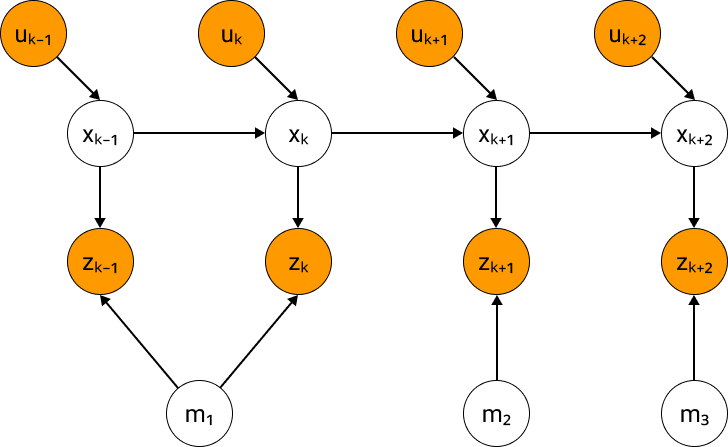
\includegraphics[width=0.5\linewidth]{img/FastSlamGraphical}
	\caption{
		This graphical description of the SLAM problem shows the assumption that the landmark estimates are all mediated through the robot path thus allowing for easier implementation by using smaller Gaussians for each landmark $m_{i}$ rather than a larger state-space vector as in EKF SLAM.
	}
	\label{fig:fastSlamGraphical}
\end{figure}

\subsection{Graph-based}
The newest paradigm to solve the offline SLAM problem are graph-based methods that essentially use a non-linear least-squares approach to compute the graph of poses best fitting the measurements. 
To this end the SLAM posterior is described as a graph of robot poses $ x_{i} $ at time $ t_{i} $ as nodes connected by soft constraints that correspond to spatial measurements $z_{ij}$ between two states.
These edges are generated in the following two cases:

\begin{equation}\label{odometryEdge}
	(X_{i}^{-1}X_{i+1})
\end{equation}

\begin{equation}\label{observationEdge}
	(X_{i}^{-1}X_{j})
\end{equation}

Here \ref{odometryEdge} corresponds to a edge based on odometry transformations by moving the robot from state $X_{i}$ to $X_{i+1}$, both of which are represented as vectors relative to the coordinate origin.
These transformations are illustrated in more detail in Fig. \ref{fig:poseGraphTransformation}.
The more interesting case is when an observation of a previously captured area occurs and a virtual measurement \ref{observationEdge} is computed, describing how the states $X_{j}$ and $X_{i}$ relate to each other according to the displacement between their observations, see Fig. \ref{fig:poseGraphOptimization}.

\begin{figure}
	\centering
	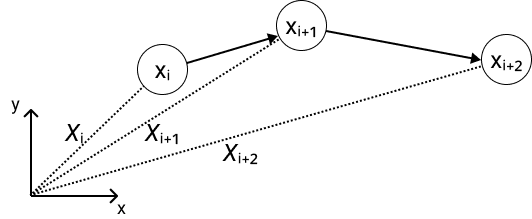
\includegraphics[width=0.6\linewidth]{img/PoseGraphTransformation}
	\caption{
		The graph of robot poses connected to each other by odometry measurements. To calculate the relative movement between two nodes each node can be represented as a matrix $X_{i}$ describing how it is transformed relative to the global coordinate frame.
	}
	\label{fig:poseGraphTransformation}
\end{figure}



This approach marginalizes any data about the map other than the correspondence of poses to primarily focus on solving the robot path. 
Given the pose-graph the goal is to compute the node configuration that minimizes the error between predicted edges, see \ref{observationEdge}, and actual measurements 
$
\langle
\begin{matrix}
	z_{ij},  \Omega_{ij}
\end{matrix}
\rangle
$, with the information matrix $\Omega_{ij}$ describing the measurement noise.

Equation \ref{leastSquares} describes this optimization process, with the error function $e_{ij}$ defined as any non-linear function essentially calculating the difference between estimate and true measurement for any pair of nodes. 
Once the optimal pose-graph is constructed the map data is rendered given known poses thus reducing the problem to simple mapping\footcite{grisetti2010graphSLAM}.

\begin{equation}\label{leastSquares}
	x* = argmin_{x} \sum_{ij}e_{ij}^{T} \Omega_{ij} e_{ij}
\end{equation}


\begin{figure}
	\centering
	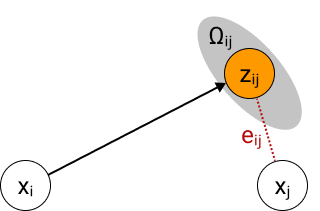
\includegraphics[width=0.4\linewidth]{img/PoseGraphOptimization}
	\caption{
		This pose-graph with two nodes describes how any pair of nodes are related to each other given a measurement. The measurement $ z_{ij} $ corresponds to how the node $x_{j}$ should be placed relative to node $x_{i}$ given that each of them share a similar observation. As seen in the figure this is not the case, thus demanding for the error $e_{ij}$ to be minimized. In other words, by moving the node $x_{j}$ closer to the optimum minimizes the error and corrects the pose-graph. \footcite{grisetti2010graphSLAM}
	}
	\label{fig:poseGraphOptimization}
\end{figure}


\section{Graph-SLAM topology}
%!!!!!! Front-End Backend Trennung ist nur bei graph based der Fall
Most modern graph-based SLAM systems are partitioned into the following modules:
\begin{itemize}
	\item A front-end in charge of abstracting sensory input by performing feature extraction as well as data association, further described in Section \ref{dataAssociation}. Essentially it constructs the pose-graph and feeds it into the back-end.
	%Furthermore it is responsible for associating corresponding features over multiple measurements, which is typically referred to as short-term data association. Long-term data association or loop closure therefore aims to link current measurements to previously observed features thus  correcting accumulated odometry errors as well as adapting the global topology. 
	\item A back-end performing pose-graph optimization based on the abstracted data fed in by the front-end. The back-end also provides positional information about nodes to the front-end thus supporting loop closure detection. 
\end{itemize}

While the front-end remains application specific as the data abstraction depends on the sensors utilized by the robot, the same back-end can be applied for many different scenarios as the pose-graph optimization essentially represents a squared-error minimization and many elaborated algorithms such as Gauss-Newton can be utilized.

%and is implemented by least-square solving algorithms such as gradient decent 

%auch in section graph based schieben
\section{Data Association}\label{dataAssociation}
%While many aspects of the front-end remain application specific each SLAM system typically contains modules for data association in the two ways.
One key trait that all SLAM paradigms posses is to recognise similarities in measurements and correct the incremental odometry error after revisiting previously mapped areas. This process is referred to as loop-closing or long-term data-association and reduces the uncertainty of pose and map estimates thus qualifying it as a integral part of any SLAM problem. 

While loop-closures aim to detect large correspondences in the global map, short-term data-association is responsible for associating corresponding features over multiple measurements which helps establishing the pose-graph. 

\section{Hierarchical Pose-Graphs}
While building the pose-graph can be computed with relatively low effort, performing loop-closures is a computational heavy process. Which makes graph-based online SLAM solutions difficult to implement as robot state and map need to be estimated in real-time scenarios. To facilitate the data association process, the global map is partitioned into sub-maps thus allowing data-associations to be calculated only in parts of the graph the robot is currently present. 

\section{Comparison of SLAM Paradigms}
%The previous sections explained the basic structure of the three main approaches to the SLAM problem with the Extended Kalman Filter being the most mature. 

%In its basic implementation the algorithmic complexity of EKF-SLAM is tightly coupled to the size of the covariance matrix which grows quadratically as more landmarks are observed. Furthermore local linearization as utilized in this approach has many disadvantages as results can be very inconsistent. To solve this efficiency problem many optimization approaches have been implemented in the past years\footcite{bailey2006simultaneous}.

%Particle filtering methods such as Fast-SLAM solve many issues found in the EKF as they directly incorporate a non-linear process model instead of performing linearization beforehand. Although the number of particles needed may increase dramatically Fast-SLAM still performs well with linear  time-complexity which may even be improved by implementing a balanced binary tree to organize particles as Montemerlo\footcite{montemerlo2002fastslam} suggests. 

%Contrary the relatively modern graph-based approach inherently aims to solve the Full-SLAM problem as it performs pose-graph optimization on the whole graph. The main benefit of this solution is the decoupling of front- and back-end which allows it to be used in many different scenarios. 
%Although its basic implementation performs offline many newer approaches adjust the pose-graph in real-time which makes such solutions relatively similar to EKF-SLAM. 


The Extended Kalman Filter is a mature approach to the SLAM problem and has been implemented many times in different types of applications. However it does not only lack computational efficiency in its original implementation, see. Tab. \ref{tab:slamComparison}, but also has shown to be very problematic concerning consistent solution and robust data-association. 
These problems stem from the algorithm definition itself, firstly as local-linearization of non-linear problem impairs the system to reach complete convergence, e.g. all landmark uncertainties converging to zero. Secondly the data-association model of EKF assumes all landmarks to be fully identifiable from any point of view, which cannot be guaranteed in most real-life scenarios and renders data-association very fragile.
Fortunately the EKF has been improved and optimized to address some of the aforementioned issues\footcite{bailey2006simultaneous}.

Another paradigm proposed was Particle Filtering which essentially applies a survival of the fittest model to robot poses. Solutions like Fast-SLAM optimize MCL algorithm by decoupling landmarks and estimating them through individual EKFs. 
The main benefit of this solution is the utilization of a non-linear model and ability to perform even with non-Gaussian distributions. 
Although its computationally more efficient compared to the previous approach, one problem is the need for large amounts of particles to achieve high accuracy. Montemerlo suggest implementing a balanced binary tree to store and organize particles which improves the complexity of the algorithm to $O(J  \log  M)$ with $J$ representing the amount of particles and $M$ being the number of landmarks\footcite{montemerlo2002fastslam}.

Lastly mentioned was the graph-based approach to SLAM which has grown significant popularity due to its versatility and reusability in different applications. The robot posterior is modelled as a sparse pose-graph which is optimized using a least-squares algorithm and is solved offline after the whole robot path has been captured. Some newer algorithms try to manipulate the pose-graph in real-time to establish a graph-based online SLAM solution\footcite{stachniss2016simultaneous}.


\begin{table}[]
	\centering
	\begin{tabular}{|l|l|l|}
		\hline
		\textbf{Approach}   & \textbf{Problem}    & \textbf{Time Complexity} \\ \hline
		\textbf{EKF}        & online SLAM         & $O(M^{2})$               \\ \hline
		\textbf{Fast-SLAM}  & full \& online SLAM & $O(J M)$                 \\ \hline
		\textbf{Graph SLAM} & full  SLAM          & $O(|V| + |N|)$           \\ \hline
	\end{tabular}
	\caption{The three main SLAM solution paradigms in basic implementation compared by their computational complexity. Note that the quadratic time complexity of the EKF approach is caused by quadratically extending the covariance matrix as landmarks $M$ are added and updated throughout mapping \footcite{durrantSlam2006}.
	For Fast-SLAM the complexity concerning just the particles $J$ stays linear, however during every resampling step each particle including all landmark estimate $M$ contained within need to be copied\footcite{montemerlo2002fastslam}.
	Lastly the back-end for most graph SLAM solution is based on least-squares error minimization of the pose graph with $|N|$ nodes as robot poses and $|V|$ vertices as measurements between nodes thus rendering the computational complexity to be  $O(|V| + |N|)$ without utilized hierarchical pose-graphs as studied by Korovko and Robustov\footcite{korovko2021partial}. 
}
	\label{tab:slamComparison}
\end{table}

\section{SLAM in Autumn}

\begin{figure}
	\centering
	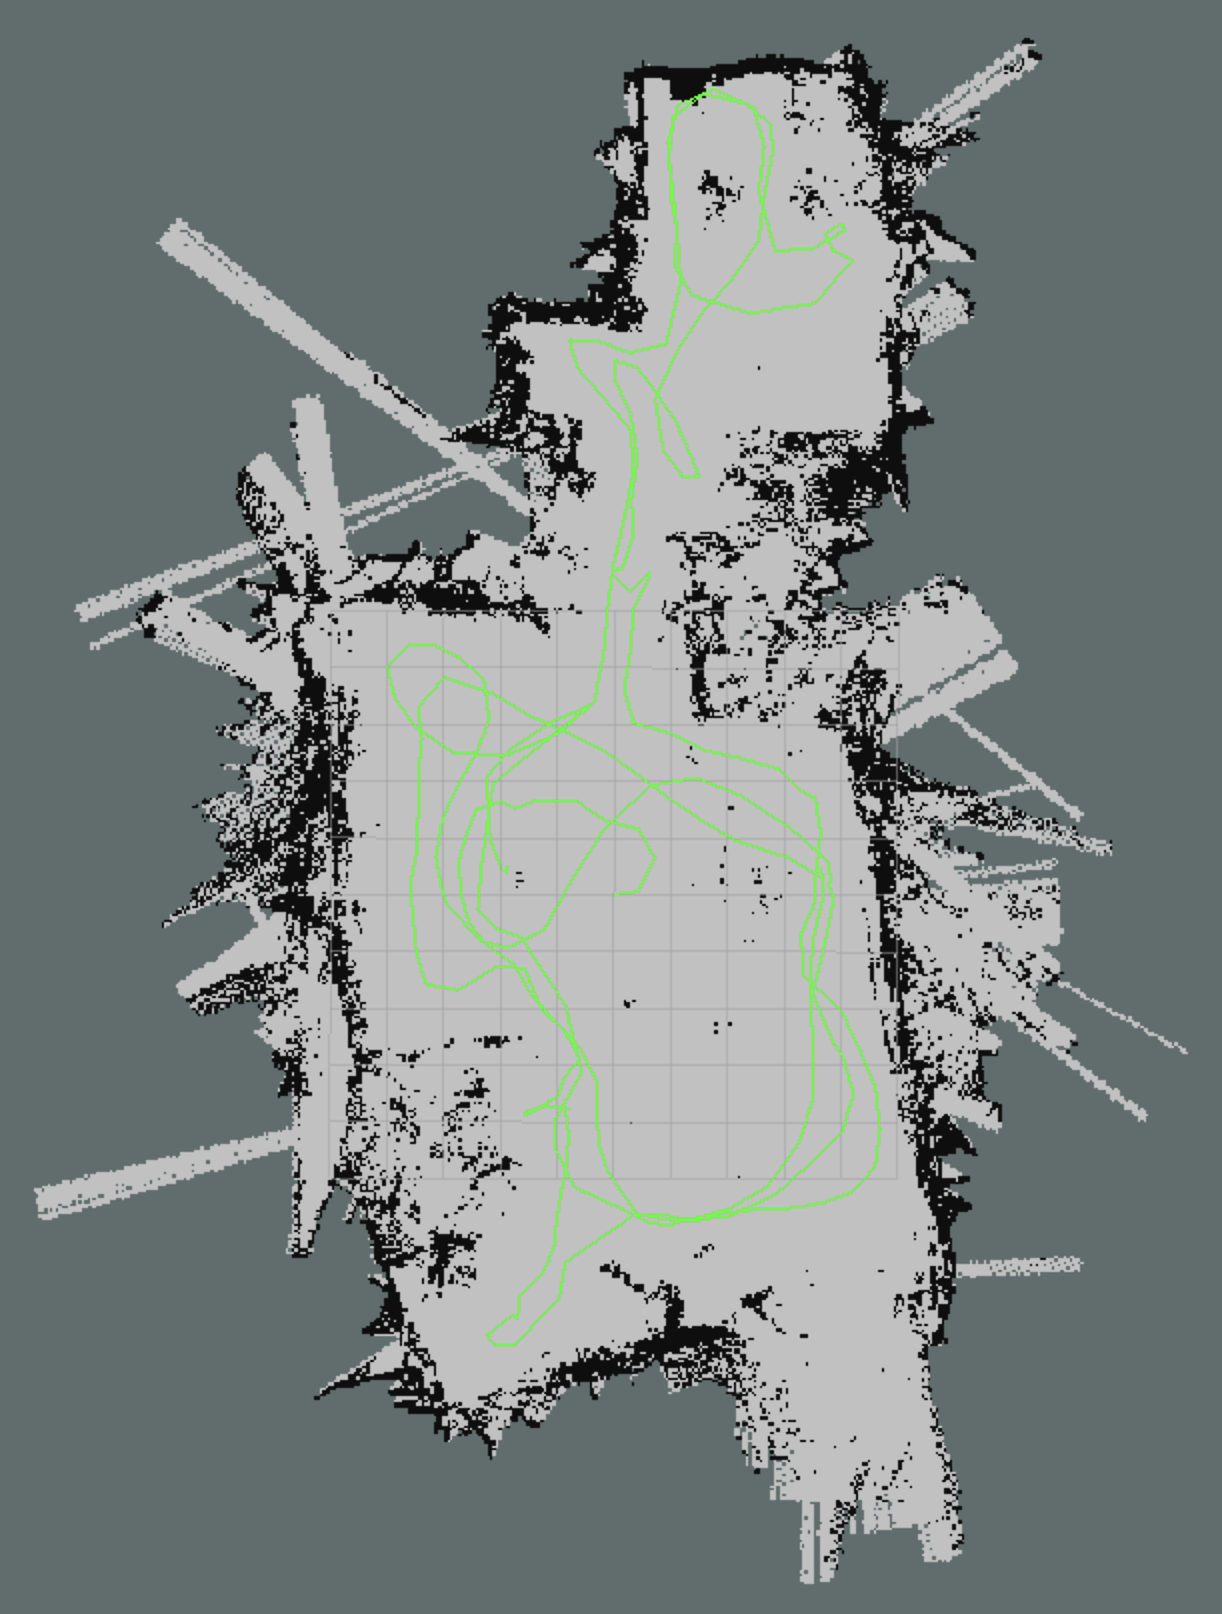
\includegraphics[width=0.8\linewidth]{img/airlabMap}
	\caption{
		Occupancy grid of the AIRLab at the HTBLuVA Wiener Neustadt including the path pursued by the drone as it got carried through the laboratory. The map as seen above is of low quality including many artefacts, sensor noise as well as misaligned proportions.
		Although the main room is poorly mapped with many error, the smaller workshop at the top is depicted relatively accurate.
	}
	\label{fig:AirLABmap}
\end{figure}

As localization and mapping data is utilized to perform real-time path-planning as well as drone control these modules are a crucial part of the Autumn Drone, thus requiring a algorithm that solves the online SLAM problem in a efficient manner while maintaining compatibility to the hardware in use. This restraints the solution in question to perform visual SLAM supporting stereo images and 6DoF-Odometry. 
While remaining within the package-space of ROS this reduces the number of potential algorithms to the following graph-based SLAM solutions:
\begin{itemize}
	\item \href{https://github.com/raulmur/ORB_SLAM2}{ORB-SLAM2}
	\item \href{https://github.com/lrse/sptam}{S-PTAM}
	\item \href{http://introlab.github.io/rtabmap/}{RTAB-Map}
	\item \href{https://felixendres.github.io/rgbdslam_v2/}{RGBDSLAMv2}
\end{itemize}

ORB-SLAM2 and S-PTAM where not selected as both approaches do not provide online occupancy grids as ROS-Topics which makes them infeasible to use and incorporate with the path-planning module of Autumn. Furthermore they do not propose a memory-management strategy thus potentially making loop-closure processing within large maps cumbersome. 

The algorithm chosen to be used for Autumn was RTAB-Map as incorporating stereo-images and external odometry is supported out-of-the-box and a variety of outputs such as 2D and 3D occupancy grids as well as a dense point cloud are offered. 
As loop-closure detection algorithm with memory management was the primary goal of RTAB-Map, it qualifies for usage in large-scale environments during long mapping sessions.
Since its publication in 2013 this algorithm has been extended and improved to support stereo- or RGBD-footage, 2D as well as 3D Lidar data and provides nodes for processing visual or lidar based odometry if no other external topic is available. 
For Autumn this approach was implemented by providing the stereo-image stream as well as visual odometry data from the Stereolabs ZED2 thus yielding in multiple occupancy grids, robot paths as visualized in Fig. \ref{fig:AirLABmap}.

Although RGBDSLAMv2 does not fully qualify to be considered in this project as it only works with RGBD-Cameras like the XBOX Kinect or Intel RealSense it is worth mentioning as it provides a 3D occupancy grid and a dense point-cloud similar to RTAB-Map.\footcite{labbe2019rtab}

%\section{Application Scenarios}
%
%\subsection{Map Acquisition}
%
%\subsection{Black-Box Localization}
%
%\subsection{Continuos Map Exploration}
%
%
%\section{2D SLAM}
%
%\subsection{Evidence Grid-based SLAM}
%
%\subsection{Graph-based SLAM}
%
%\subsection{Feature-based SLAM}
%
%
%\section{3D SLAM}
%
%\subsection{Visual SLAM}
%
%\subsection{Graph-based SLAM}
%
%
%\section{Obtaining Odometry}
%
%\subsection{Wheel Encoder Odometry}
%
%\subsection{Visual Odometry}
%
%\subsection{Visual Inertial Odometry}

\section{Topics not mentioned in this Chapter}
The SLAM problem is a highly diversified field of study with many different concepts not only concerning one paradigms adaption to other use cases than originally mentioned but also diving into the exact implementations of any of its components. Due to this abundance of concepts and algorithms it would be infeasible to characterize every one of them. 
However for the intrigued reader the author suggests the following topics and resources for further reading:
\begin{itemize}
	\item Particle Filtering for grid-based SLAM\footcite{grisetti2005ParticleGrid}
	\item Visual SLAM approaches. A wide range of literature on this topic is provided by the \href{https://vision.in.tum.de/research/vslam}{Technical University in Munich (TUM)}.
	\item Graph-SLAM frontends using different data association approaches for visual SLAM such as feature based matching like RANSAC\footcite{Jia2018FeatureMatching} or point-to-point matching like ICP\footcite{Horn1988ICP}. 
	\item Mapping in dynamic environments capable of comprehending moving obstacles within the environment\footcite{wang2003dynSLAM}
	\item SLAM with multiple robots\footcite{gutmann2003IncrMapping}
\end{itemize} 




\filbreak
	
	\chapter{Path Planning}

\textbf{Author: Fabian Kleinrad} 

A crucial part of autonomy in robotics are the means for planning ahead movements in a cooperative manner with the environment. Methods to accomplish this, are generally referred to as path planning algorithms. This chapter is going to focus on exploring different kinds of approaches to path planning and evaluate which approach is most fitting to be used in a real-time, high-dimensional use case present in the autumn project.


\section{Types of Path Planning}

The problem of finding an optimal path between two points is an old one.
The first proposed solution was the Dijkstra's algorithm. However, with steadily evolving computer science the challenges to be mastered by such algorithms got harder and harder. That's the reason why over the last years the simple principle of the Dijkstra algorithm has branched out specializing and excelling in certain real-world applications.
\footcite{Pan2020}

\subsection{Sampling-based Algoritms}

In motion planning, sampling-based algorithms can be differentiated to other kinds of approaches, by the way, they explore their environment. sampling-based algorithms such as the probabilistic road map algorithm or the rapidly exploring random tree use a random point in their reference space and expand in that direction. This random point is considered a sample.

\subsection{Multiple-Query and Single-Query}

The term multiple-query refers, in connection with path planning Algorithms, to the feasibility of deriving a variety of different paths, without the need of rerunning the algorithm. In contrast, single-query algorithms are only able to compute one path at a time.\newline
Use cases for Multiple-Query Algorithms would be unchanging environments. The reason for that, by generating an extensive grid of connections to be able to calculate a multitude of different start/goal combinations  more computational time is needed.\newline
Single-Query approaches focus on performance instead of reuse-ability, which makes them ideal for dynamic domains. 
\footcite{Bekris2003}
\footcite{stackexchangeMultiSingleQuery2019}

\section{PRM}

Probabilistic RoadMap is a path planning algorithm tailored to multi-query applications. It is considered one of the most influential sampling-based path planning algorithms. 

The algorithm can be broken down into two phases. The first phase, which is referred to as the pre-processing phase, starts with an empty graph. At first, it samples n random points and adds them to a set of vertices if they are located in space free from obstacles. After constructing a set of n vertices, it attempts connections between a random vertex and its neighboring nodes in a predefined radius. This connecting of to vertices is realized with a simple straight-line connection. All collision-free connections between vertices and their respective neighbors are added to a set of edges. The result of this pre-processing phase is a roadmap, with the number of sampled points determining the quality of to be calculated paths. 
\footcite{Karaman2011}

Upon finishing the initial construction phase of a roadmap, like the one depicted in figure 8.1, start/goal combinations can be processed. 
The actual path finding in the generated graph is handled by other non-sampling-based path finding methods such as A*.\newline
With the PRM focusing on a multi-query approach it is possible to calculate an arbitrary number of different paths without the need to construct a new graph.

\begin{figure}[h]
	\centering
	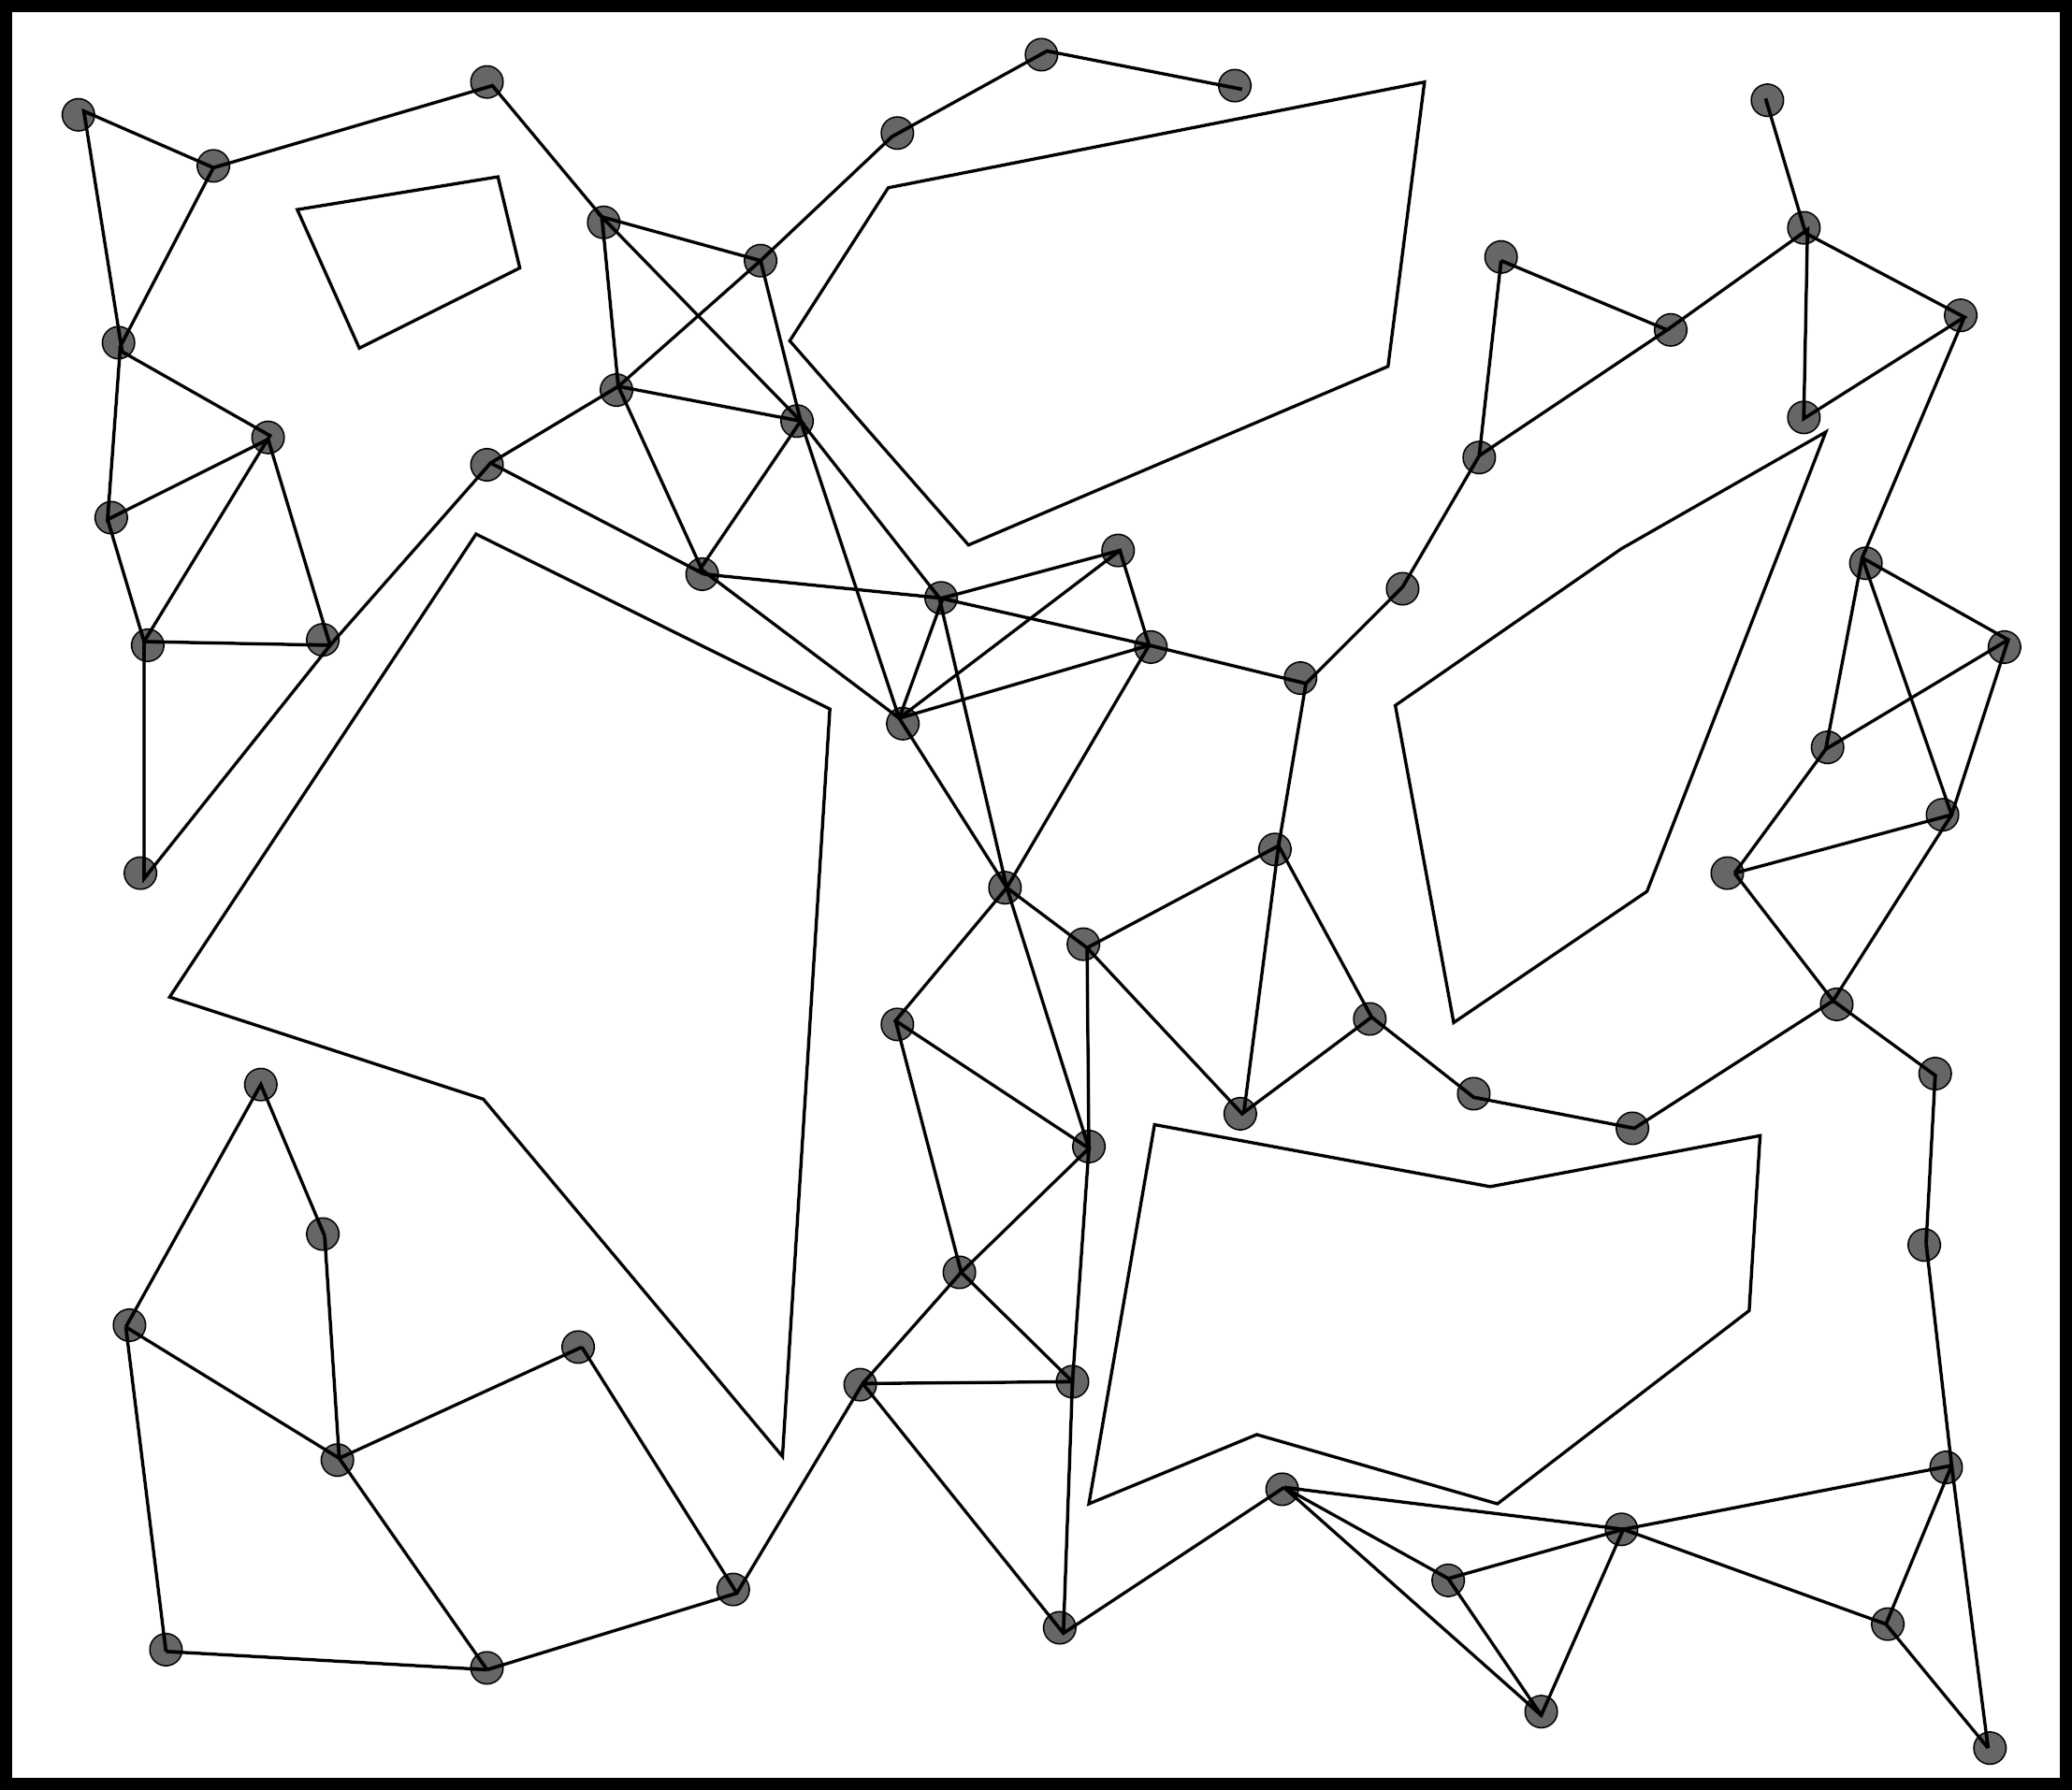
\includegraphics[width=0.7\linewidth]{img/PRMRoadmap}
	\caption{Example of a roadmap in two dimensional space constructed by the PRM algorithm.}
	\label{fig:path_planning_prm}
\end{figure}

\section{RRT Algorithm}

Rapidly exploring random tree is a path planning algorithm, that can be categorized as sampling-based and single-query. In the field of sampling-based path-finding algorithms is it considered together with the PRM the most influential. RRT works by constructing a tree of possible trajectories. Therefore it is first required to define an initial vertex, much like a root. After each following iteration, a random sample is taken from the space that is considered free from obstacles. After generating a random vertex, the nearest neighboring point in the tree is searched for. The closest node is then used as a pivot point and a new vertex is constructed a predefined distance away from the nearest node in the direction of the random sample. Thereafter it is attempted to connect the new vertex with the nearest. If this straight-line connection can exit without colliding with obstacles it is added to the set of edges. This procedure is depicted in figure 8.2. The algorithm ends when a new node is within the predefined distance away from the goal point. 
\footcite{Karaman2011}

The name rapidly exploring random tree stems from the tree-like structure constructed, like the one you can see in figure 8.2 when exploring spaces This approach to path planning makes it possible to explore rapidly changing environments efficiently.


\begin{figure}[h]
	\centering
	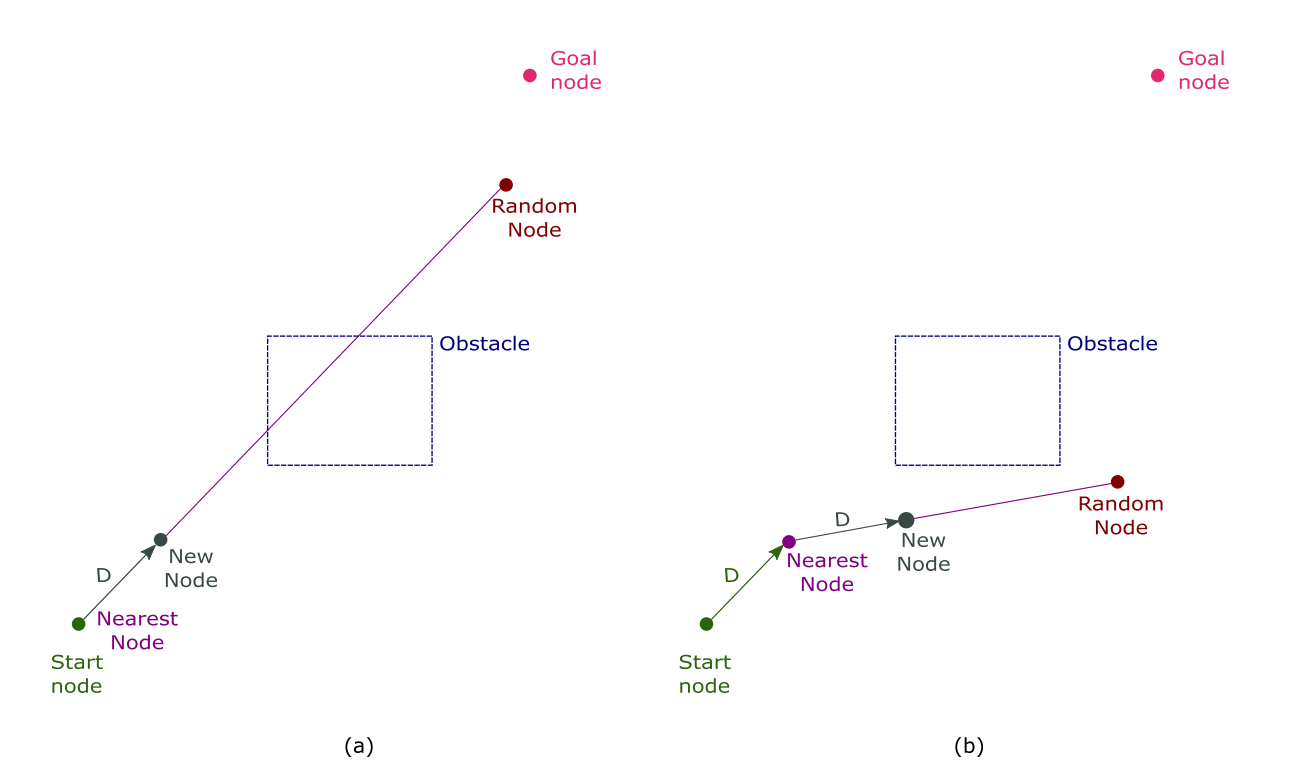
\includegraphics[width=0.9\linewidth]{img/rrtIteration}
	\caption{Visualization of the first two iterations (a), (b) when an rrt algorithm is exploring a simple 2d space wihttps://robotics.stackexchange.com/questions/18433/difference-between-single-query-and-multiple-query-algorithmsth an obstacle present. D referring to the predefined distance between vertices.\footcite{Zammit2018}}
	\label{fig:path_planning_rrt}
\end{figure}

\section{A* Algorithm}

The A* algorithm is a simplistic and reliable method compared to other path-planning techniques. Therefore it is nowadays prevalently used in a variety of different applications.\footcite{Zammit2018}\newline
It combines heuristic properties with formal virtues of Dijkstra's algorithm. Whereas a purely heuristic approach would not guarantee that a path can be found even if a possible solution existed, the A* guarantees that the shortest path is found.\footcite{Sathyaraj2008}
A* works by trying all possible combinations like the Dijkstra algorithm in a grid or graph-based environment. With A* being based on the Dijkstra algorithm it favors nodes that are closer to the current position. Additionally, it follows heuristic principles by putting a higher priority on nodes closer to the goal. An example of what an A* search algorithm looks like in a grid-based environment is depicted in figure. 8.3.\footcite{standfordAStarComparison1997}\newline
With these properties, it can be considered an informed Dijkstra search.
  
\begin{figure}[h]
	\centering
	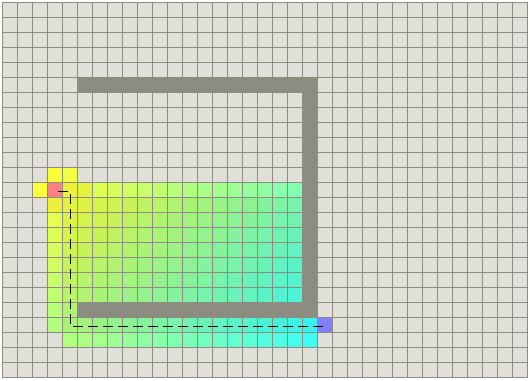
\includegraphics[width=0.7\linewidth]{img/AStarExample}
	\caption{A* path finding around a concave obstacle in a grid-based environment.\footcite{standfordAStarComparison1997}}
	\label{fig:path_planning_Astar}
\end{figure}

\section{Evaluation}

This section is going to cover the reasons behind the selection of the path-planning algorithm used in autumn. Therefor we are going to theoretically evaluate the performance of each algorithm in relation to the environment provided by the project. Additionally, we are going to focus on properties essential for accomplishing the goal set in the autumn project.

\subsection{Autumn Use-case}

There are several criteria to be fulfilled, in order to be considered a working solution for the challenge of path planning faced by Autumn.
As a means to use one of the aforementioned algorithms, they have to be suitable for a real-time, 3-dimensional application, like the one present in the project.
When working with UAVs it is critical that an optimal path is calculated reliable and in the shortest amount of time possible. 

\subsection{Comparison}

In the following comparison, we are going to look at the performance of the three different algorithms already mentioned in this chapter. Knowing that the PRM algorithm doesn't find a path on its own, it is implied from here on out that the PRM works in combination with the A* algorithm and the A* on its own is only applied with grid-based environments.  

\subsubsection{Computational time requirement}

An important requirement to be fulfilled by the path planning algorithm of the Autumn project is to require as little computational time as possible. Taking a look at the PRM algorithm, with its principle of reusing the generated graph, as a road-map, resulting in a short runtime of the algorithm, when looking at the computation of multiple paths. The best-case scenario for the PRM in this configuration would be, an A* algorithm running in a graph-based environment, with the PRM only having to do generate the graph and improve it progressively. A problem that arises is that this best-case scenario is impossible to happen in the Autumn project. Starting uneducated about the environment, like in Autumn, is the worst case for the PRM. At first, the PRM algorithm would generate a road-map in an environment where most of the obstacles are still unknown. Thereafter when the drone gets its first path to its destination it detects obstacles and expands the known space for the algorithm. With the environment changing as much as in Autumn it would be far too expensive to rewire the existing road-map around new obstacles. A* is the best-case scenario in a graph-based environment for the PRM, but what about running the A* standalone now in a grid-based environment. Grid-based environments tend to be very resource-intensive, with full coverage of the entire space. To preclude the possibility of large portions of the search being dissipated, the A* is biased towards the goal. When comparing the A* to the PRM in terms of computational speed in Autumn, A* would be superior, because of the substantial amount of time the PRM takes to generate a road-map only to discard it a few iterations later. That being said, the A* still needs to cover a vast grid, depending on the granularity of the grid. Know knowing that both the A* and PRM algorithms aren't the most efficient in the matter of short runtime, let's cover the RRT algorithm. With RRT following a graph-based and sampling-based approach like the PRM, it covers the space to be explored within a short time frame. The RRT, in contrast to the PRM, doesn't take time to construct the graph and then start to find a path. RRT searches for a path while constructing the tree-like structure. This results in the fastest computational time of all other mentioned algorithms when looking at one-time path planning. With the reference space of the algorithm in Autumn being drastically and continuously changing, it resembles a one-time use path perfectly fitted to be determined by a single-query path planning algorithm like the RRT.

\subsubsection{Scalability for high-dimensional spaces}

Thus far the application of proposed algorithms happened in a two-dimensional environment. When working with UAVs, there is the added challenge of a third dimension to be covered, in contrast to using ground-based vehicles. This added dimension imposes new challenges that the whole system has to handle, with the means to plan a path being one of the most affected.
Additional time complexity being the most crucial change when working in a higher dimension, it is essential to be as efficient as possible. The last point covered the time required for each algorithm. With most path-planning algorithms having a time complexity of \(O\left(b^d\right)\)\footcite{stackexchangeAstarTimeComplexity2019}. With A* being one of the most time-intensive.
In this equation, the variable $b$ is the branching factor and describes the number of descendants of a parent node. $d$ refers to the depth of the goal node. The worst-case scenario would be \(O\left(|V|\right)\), meaning that every vertex of the reference space has to be checked. Looking at the problem of three dimensions where the added dimension increases the number of vertices exponentially. A* being a simple approach with brute force characteristics isn't suitable for application in high dimensional spaces. 

Comparing the RRT to the A* highlights the benefits of a sampling-based approach. While the A* looks at direct neighbours to continue the search, RRT has a step range as a predefined constant. Therefore the RRT explores with a faster pace due to a rougher coverage of the space. This means in relation to higher dimensional spaces it converges more efficiently than the A*.

\subsection{Collusion}

By evaluating the potential algorithms to be used in the autumn project, the RRT came out on top. With each algorithm providing unique features best fitted for the use-case they are designed for, the problems the RRT algorithm tries to solve are the same encountered in autumn. Properties like space complexity and path quality were neglected in this comparison, due to the low importance of the project. By shifting the computation away from the drone the importance of minimum time far outweighs the required space. Furthermore, the need for an optimal path isn't required on account of the goal being to cover the whole space eventually. That being said a big drawback of the base RRT algorithm is the incapability to provide the possibility to improve on an existing path by rewiring the graph. For that, we are going to take a look at a variant of RRT the RRT* that solves this exact problem.


\section{RRT* Algorithm}

This section is going to cover the improved version of the RRT algorithm, mentioned above. The RRT* algorithm is being used in the Autumn project as the path planning algorithm. The rationale for this decision is covered in the evaluation section. 

\subsection{Concept behind RRT*}

A problem that arises when using the RRT algorithm is that finding an optimal path is impossible due to the lack of rewiring options. Therefore the RRT* algorithm was invented. 
The improved algorithm works differently when connecting a newly sampled node into the existing tree structure, which in the RRT is done by connecting the new node to its nearest neighbour. In the case of the RRT*, it calculates the cost of other possible connections stemming from the root node. Hereby a set of nodes closest to the newly sampled vertex are used as possible connection candidates. By rewiring the tree after each new node is sampled it makes it possible for a near-optimal path to be found.

\subsection{Algorithm}

The RRT* works at first the same as the RRT algorithm, it first defines a set of vertices, $V$ with the start node and an empty set of Edges, $E$. In contrast to the RRT algorithm is the runtime of the RRT* algorithm is not dependent on how fast the goal node is reached, but instead on the degree of optimization for the calculated path.
Line four to six in Algorithm 1, are the same as the base algorithm. Hereby is a random node sampled, the nearest node in relation to the random node is calculated and a new node generated. After checking if a straight-line connection is possible between $x_{nearest}$ and $x_{new}$, a set of neighbouring vertices, $X_{near}$ is initialized.
$X_{near}$ consist of nodes in the tree with a distance $D$, in relation to $x_{new}$. Thereafter $x_{new}$ gets added to the $V$. In lines 9 to 13, the cost of paths connecting the nodes of $X_{near}$ with $x_{new}$ get calculated and an edge between the node with the cheapest path, $x_{min}$ and $x_{new}$ gets added to $E$. The final stage of the RRT* is to rewire all neighbouring nodes in $X_{near}$, if the path connecting to $x_{new}$ is cheaper than the original path to the root vertex. 

\begin{algorithm}[H]
	\caption{RRT* 2011\footcite{Karaman2011}}
	\SetKwFunction{FObstacleFree}{ObstacleFree}
	\SetKwFunction{FSampleFree}{SampleFree}
	\SetKwFunction{FNearest}{Nearest}
	\SetKwFunction{FNear}{Near}
	\SetKwFunction{FCost}{Cost}
	\SetKwFunction{FCollisionFree}{CollisionFree}
	\SetKwFunction{FSteer}{Steer}
	\SetKwFunction{FLine}{Line}
	$V \gets \{x_{init}\}$\;
	$E \gets 0$\;
	\For{$i \gets 1$ \textbf{to} $n$} {
		$x_{rand} \gets \FSampleFree()$\;
		$x_{nearest} \gets \FNearest(G = (V, E), x_{rand})$\;
		$x_{new} \gets \FSteer(x_{nearest}, x_{rand}, D)$\;
		\If{\FObstacleFree($x_{nearest}$, $x_{new}$)}{
			$X_{near} \gets \FNear(G = (V, E), x_{new}, D)$\;
			$V \gets V \cup \{x_{new}\}$\;
			$x_{min} \gets x_{nearest}$\;
			$c_{min} \gets \FCost(x_{nearest}) + c(\FLine(x_{nearest}, x_{new}))$\;
			\ForEach{$x_{near} \in X_{near}$} {
				\If{\FCollisionFree($x_{near}$, $x_{new}$) $\land$ \FCost($x_{near}$) + $c(\FLine(x_{near}, x_{new})) < c_{min}$}{
					$x_{min} \gets x_{near}$\;
					$c_{min} \gets \FCost(x_{near}) + c(\FLine(x_{near}, x_{new}))$\;
				}
			}
			$E \gets E \cup \{(x_{min}, x_{new})\}$\;
			\ForEach{$x_{near} \in X_{near}$} {
				\If{\FCollisionFree($x_{near}$, $x_{new}$) $\land$ \FCost($x_{new}$) + $c(\FLine(x_{near}, x_{new})) < c_{near}$}{
					$x_{parent} \gets Parent(x_{near})$\;
				}
				$E \gets (E \backslash \{(x_{parent}, x_{near})\} \cup \{(x_{new}, x_{near})\})$\;
			}
		}
	}
	\Return G = (V, E);
\end{algorithm}

\section{RRT* Variants}

\subsection{RT-RRT*}

The RT-RRT* takes focus on real-time path planning. RT-RRT* makes it possible to reposition the root node. Using this online tree rewiring strategy makes it possible to keep the previously sampled tree.
The two core principles introduced with the RT-RRT*, are tree expansion and tree rewiring. 
At first, the Algorithm starts by initializing a root node. After each following iterations, the tree expands and rewires. This sampling lasts for a user-defined time and is followed by planning a path from the root. The length of this path is controlled by the user, by defining the number of steps the path consists of. In this phase, the agent is moved gradually towards the tree root. Thereafter, when path planning is finished and the agent is located at the position of the tree root, the position of the root is changed to the next node in the generated path. This approach enables the agent to move without the time needed to compute the whole path.
Expansion in the RT-RRT* is done similar to the base algorithm, by sampling a random node, finding its neighbor with the minimum cost-to-reach and connecting them.
The rewiring is done in the default scenario done because newly added nodes have a smaller cost-to-reach than the parent of a certain node. In the second case, rewiring is needed if the environment changes. Therefore a larger portion of the tree has to change. Hereby two different modes are utilized. The first one consists of rewiring the tree in a circle centered around the tree node. For the second option, both focused and uniform sampling is used, with the difference that it is not done for one node, but instead concentrates on patches.
\footcite{Naderi2015}

\subsubsection{RT-RRT* in Autumn}

When applying the concept of the RT-RRT* to Autumn it would seem a good idea. Taking a closer look uncovers that the proposed RT-RRT* only works efficiently in environments with limited changes. Rewiring the tree, done in the case of a dynamic obstacle changing, doesn't make sense when the obstacle referred to covers a large portion of the space. This being the case in Autumn, because contrary to the examples in the paper covering the RT-RRT* is the algorithm not educated about the environment. Only while moving are obstacles and boundaries discovered In general the RT-RRT* is using concepts of road-maps like the one generated in the PRM algorithm and applying it to the RRT* algorithm.  

\subsection{Smart-RRT*}

Smart-RRT* focuses on solving the problem imposed when using the RRT* algorithm. With the slow convergence rate of the RRT* towards an ideal path, it takes up to an infinite amount of time to reach the most optimal path. Therefore Smart-RRT* utilizes two techniques, path optimization and intelligent sampling, in an effort of accelerating the rate of convergence. 
It works the same as the base algorithm till the first path is found. From there on out it applies path optimization and intelligent sampling. Path optimization works by interconnecting nodes in the found path that are directly visible. This leads based on triangular inequality to a shorter path. The reconnected nodes are then used as biased points for intelligent sampling. Intelligent sampling samples new points based on a bias generated from finding a shorter path. The result is a greater node density in the area of critical points on the path, mostly located around obstacles. 
\footcite{Islam2012}

\subsubsection{Smart-RRT* in Autumn}
Using Smart-RRT* improves the rate of convergence and time to reach an optimal path drastically. This makes one wonder why not use this improved version of the implemented algorithm in the project. When looking at this it is important to keep the goal in mind the autumn project aims to reach. Which is, to capture an environment in form of a 3-dimensional model. Therefore it is unnecessary to compute an optimal path. The whole space is going to be covered eventually which would only be a waste of computational power to invest in additional path optimization. 
	\chapter{Custom Parts}

\textbf{Author: Fabian Kleinrad} 

This chapter is going to take a look at the practical side of the autumn project. When working with hardware there is the inevitable need for parts fit for the underling application. In case of autumn, with the Matrice 100 being in the center of the project the need arises to design and manufacture parts in order to make the hardware portion in autumn come together without any complication and potential weak points in the final product.

\section{Reasons}

The goal of the autumn project being as innovative and unique in terms of methods used in the realization of the project, parts needed are either not readily available or not compliant with the budget. Another difficulty are parts too specific for there to be any commercially available. Therefor to guaranty the reusability and reliability of the final product, methods to design and produce parts specifically tailored to the needs in the autumn project have to be utilized.

\subsection{Camera Mount}

Autumn conquers the problem of mapping an environment with the use of a drone. Therefore it is necessary to attach the camera used to capture the surrounding to the drone that allows it to move through that space. In case of autumn the camera being used is a ZED2i, which needs to be securely attached to an Matrice 100. Additionally to the cost factor and accompanied risk of damaging the hardware in use, the positioning and angle are important properties to consider. For that reason a commercial solution is precluded.

\subsubsection{First approach}

When working with the principle of fast prototyping, the drawback of first approaches being incomplete is inherit. Following this principle lead to attaching the ZED2i to the Matrice 100 with the help of zip ties. Rational for this decision being the reliability and strength of zip ties which allowed the camera to be secured tightly. This was important because of the need to test segments of the autumn project, worked on separately and isolated from one another. With taking simple and easy to realize steps it enables the project to progress more smoothly and without the need for other sub-areas to be set on hold because of long tedious planing and manufacturing periods of parts like an custom camera mount for a drone.

\subsubsection{Problems without a Mount}

After a period of testing with a prototype problems arise with the need of correction. In case of an, what most people consider a work-around rather than a solution to the problem of mounting a camera, they can be, in case of this application, divided in two categories.
\newline The first aspect to consider when mounting a camera to a drone is its field of view. With UAVs hovering above ground an downward pointing angle is needed in order to be able to capture details close to the ground.  

\begin{figure}[h]
	\centering
	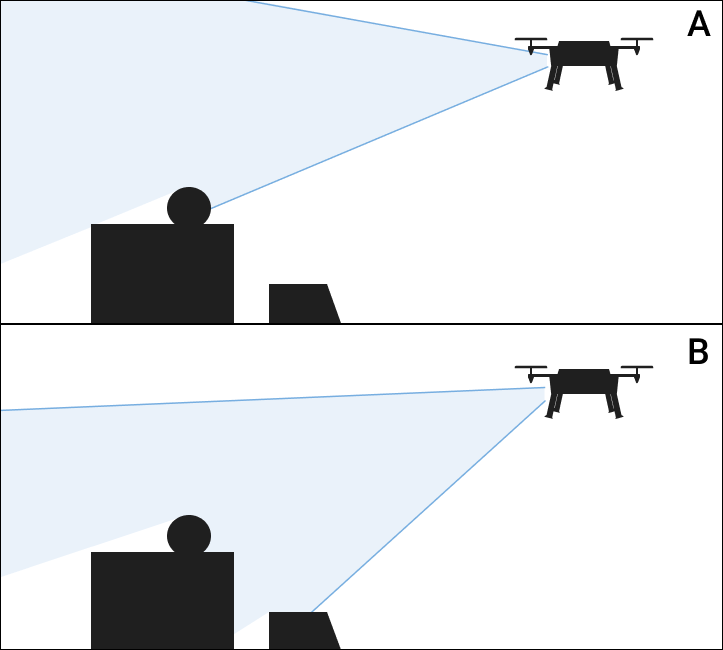
\includegraphics[width=0.7\linewidth]{img/FieldOfView}
	\caption{Depiction of the FOV for cameras mounted at different angles on a drone.\newline A: camera mounted vertically, B: camera mounted with a downward pointing angle.}
	\label{fig:custom_parts_FOV}
\end{figure}

Using zip ties results in the camera being mounted parallel to the ground. This leads to overlooking obstacles located below the field of view. This can be seen in figure 11.1 A. Adjusting the angle to be able to see as much as needed directly in front of the drone an the larger portion whats below the drone. Having the ability to capture obstacles directly in front of the drone is necessary, when wanting to be able to successfully let the drone navigate an environment autonomously. Therefor is a zip-tie solution valid, but far from optimal. A result of having a camera mounted parallel to the ground is the need to hover at a closer distance to the ground, which is potentially dangerous considering that in autumn we are not able to capture obstacles directly below the drone.

The second problem that arises when not using a mount fitted for use with, in case of autumn the ZED2i, is that the camera is not perfectly leveled. This portraits a major flaw when using a uneven camera together with a slam algorithm. Slam uses odometry data for localization and alignment of the ground plane. If the camera is slightly tilted when starting the algorithm and without manual adjustment the ground plane is going to be offset on one or multiple rotational axis. This results in the 3D model being a incorrect representation of reality. This phenomenon can be observed in Figure 11.2.

\begin{figure}[h]
	\centering
	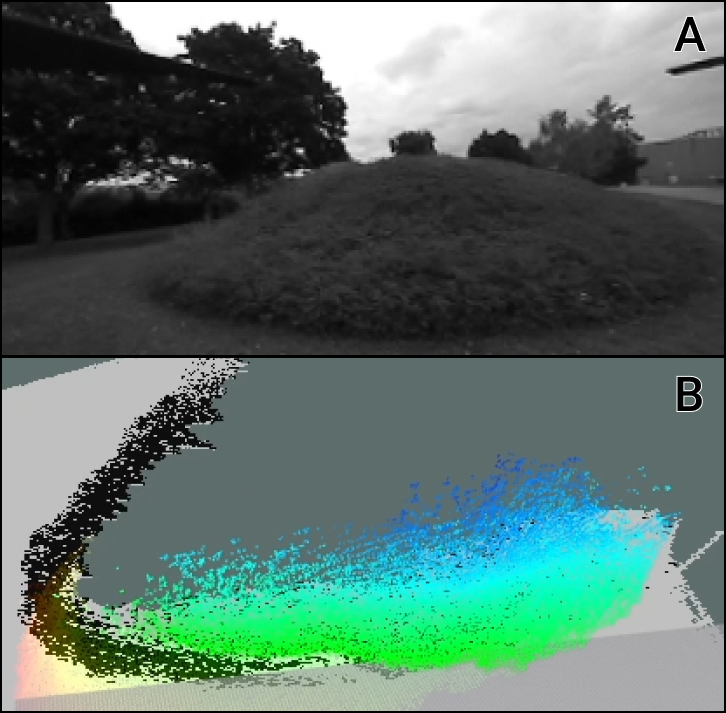
\includegraphics[width=0.5\linewidth]{img/MisalignedOdom}
	\caption{Resulting point cloud of unleveled camera with invalid odometry start data.\newline A: real life footage of the obstacle, B: tilted scan of the obstacle}
	\label{fig:custom_parts_misalignedOdom}
\end{figure}

\subsubsection{Design Process}

The solution to the aforementioned problems being a mount securing the ZED2i to the Matrice 100. Additionally to the specific characteristics the mount has to fulfill, the ZED2i is the newest model with commercial products like mounts not being available. Therefor, to attain this custom mount design and manufacturing methods have to be used. 
The design portion is done with the help of a CAD Software. CAD standing for Computer Aided Design, meaning that rather complex designs can be realized in a short amount of time and less effort than doing it the traditional way. The software used in the autumn project is Fusion360, due to its option for a free license and previously acquired knowledge working with this software. 
The mount had to perfectly fit the camera to ensure the safety of camera and drone. Therefor it is necessary to take measurements, which then are used to shape the design of the 3D-model. In Fusion360 this can be best realized using parameterized design. 

\begin{figure}[h]
	\centering
	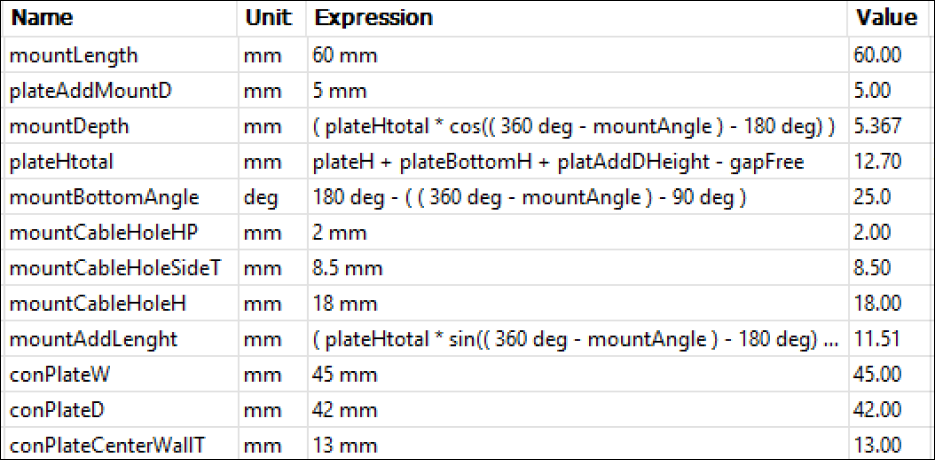
\includegraphics[width=0.7\linewidth]{img/Parameter}
	\caption{Excerpt of parameters used for the autumn camera mount design}
	\label{fig:custom_parts_parameter}
\end{figure}

Figure 11.3 depicts this concept of making the design dependent on parameters which can be easily adjusted. This allows for corrections to be made after the design processed is finished. Without linking sketches to parameters alterations would be time consuming and would result in an model clouded with sketches overriding previous adjustments. Furthermore changes affecting complex areas in the part lead to artifacts, which when removed take more time than redesigning the part in when applied to simple, one component models, like the mount in autumn. An important property in case of the autumn camera mount is the angle of the camera relative to the drone. This design principle makes it possible that changing the angle only means changing a number in a text-field, which implies the change of a number of different dimensions of the part. 
Fusion 360 additionally comes with the capability of rendering the resulting model, in order to get a feel for how it would look in physical form.

\begin{figure}[h]
	\centering
	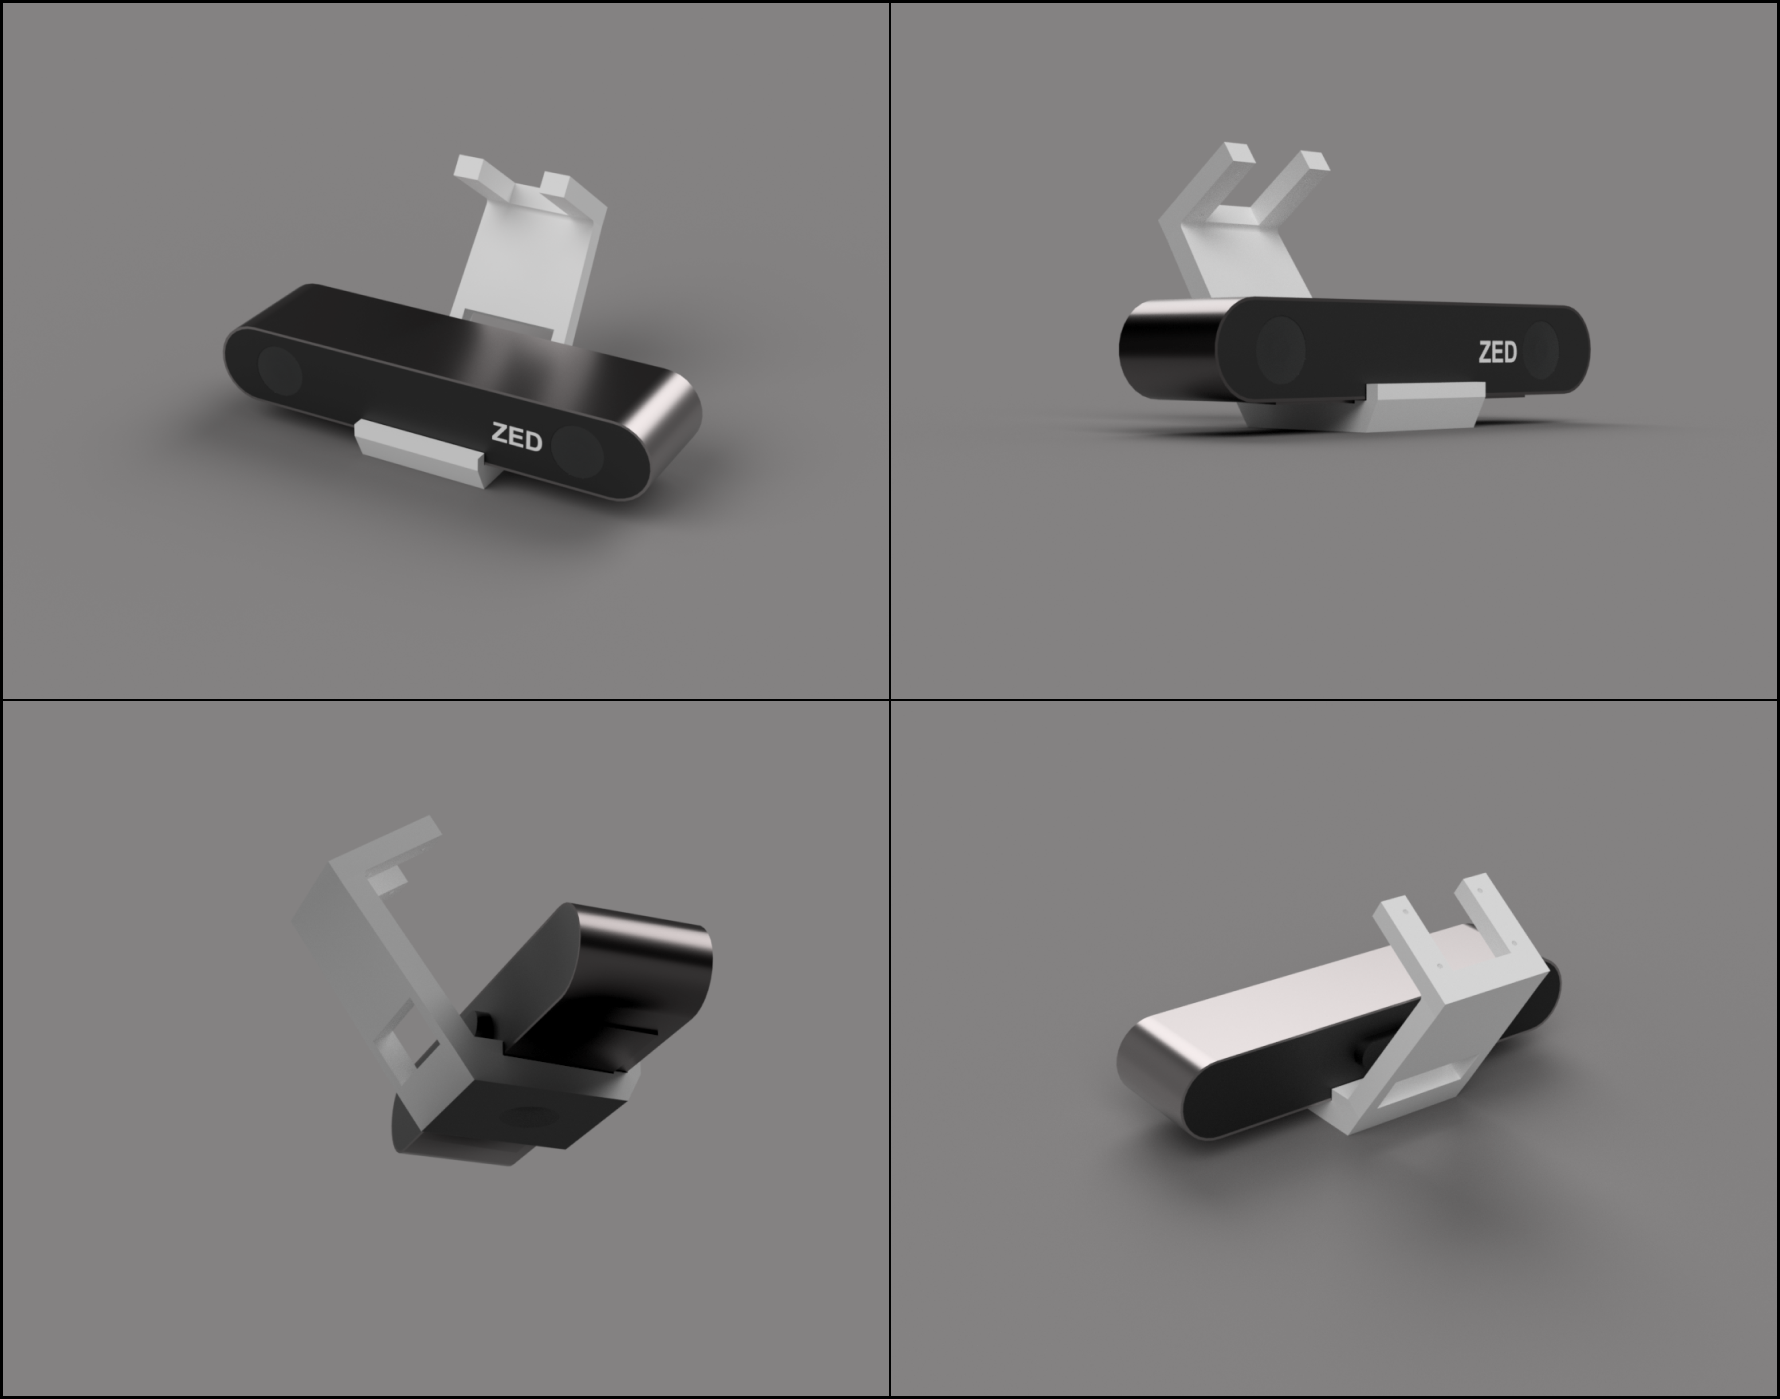
\includegraphics[width=0.6\linewidth]{img/MountRender}
	\caption{Render of the 3D-model for the camera mount attaching the ZED2i, also modeled and visible in the render, to the Matrice 100.}
	\label{fig:custom_parts_mountRender}
\end{figure}

\subsubsection{Manufacturing}

For the purpose of converting the 3D-model to an physical object, the simplest and most time efficient method is to utilize 3D-printing. Nowadays 3D-printing is a wide spread technique to make ideas reality with little time and money. Therefor it is an optimal solution for the autumn project. 
When going from a 3D-modeled design to an 3D-print a slicer is needed to convert the 3D-object to code the printer understands. With most 3D-printers printing in 2.5 dimensions, meaning that only the x and y axis move freely while the z only adjusts its height once a layer is finished. This principle is reflected in the resulting file once a 3D-model is sliced. The gcode consits of an header, defining settings for the print and a sequence of lines following it. A line of this gcode file would look like this: 
\[G1\ X120.95\ Y101.653\ E1.17355\]
The first part consisting of the identifier $G$ and a number, marks which command should be executed. In case of $G1$ it's "move in a straight line". Following the command specifier are parameters, for this example the x and y end position is needed to draw a line. Additionally marked with the identifier $E$, is the flow rate defining how much filament is going to be extruded when moving to the given position.

The final step to attaining the physical form of a gcode file, is printing it using a suitable 3D-printer. Autumn uses an Creality Ender 5, because of it's readability and print quality. Furthermore the choice of the correct filament for an successful 3D-print is needed. For a part, like the camera mount, which isn't under big stresses and no large forces are applied to it, filament like acrylonitrile butadiene styrene, commonly known as ABS, isn't needed. Therefor the most widely used filament, polylactide is most fitted for this print.

\begin{figure}[h]
	\centering
	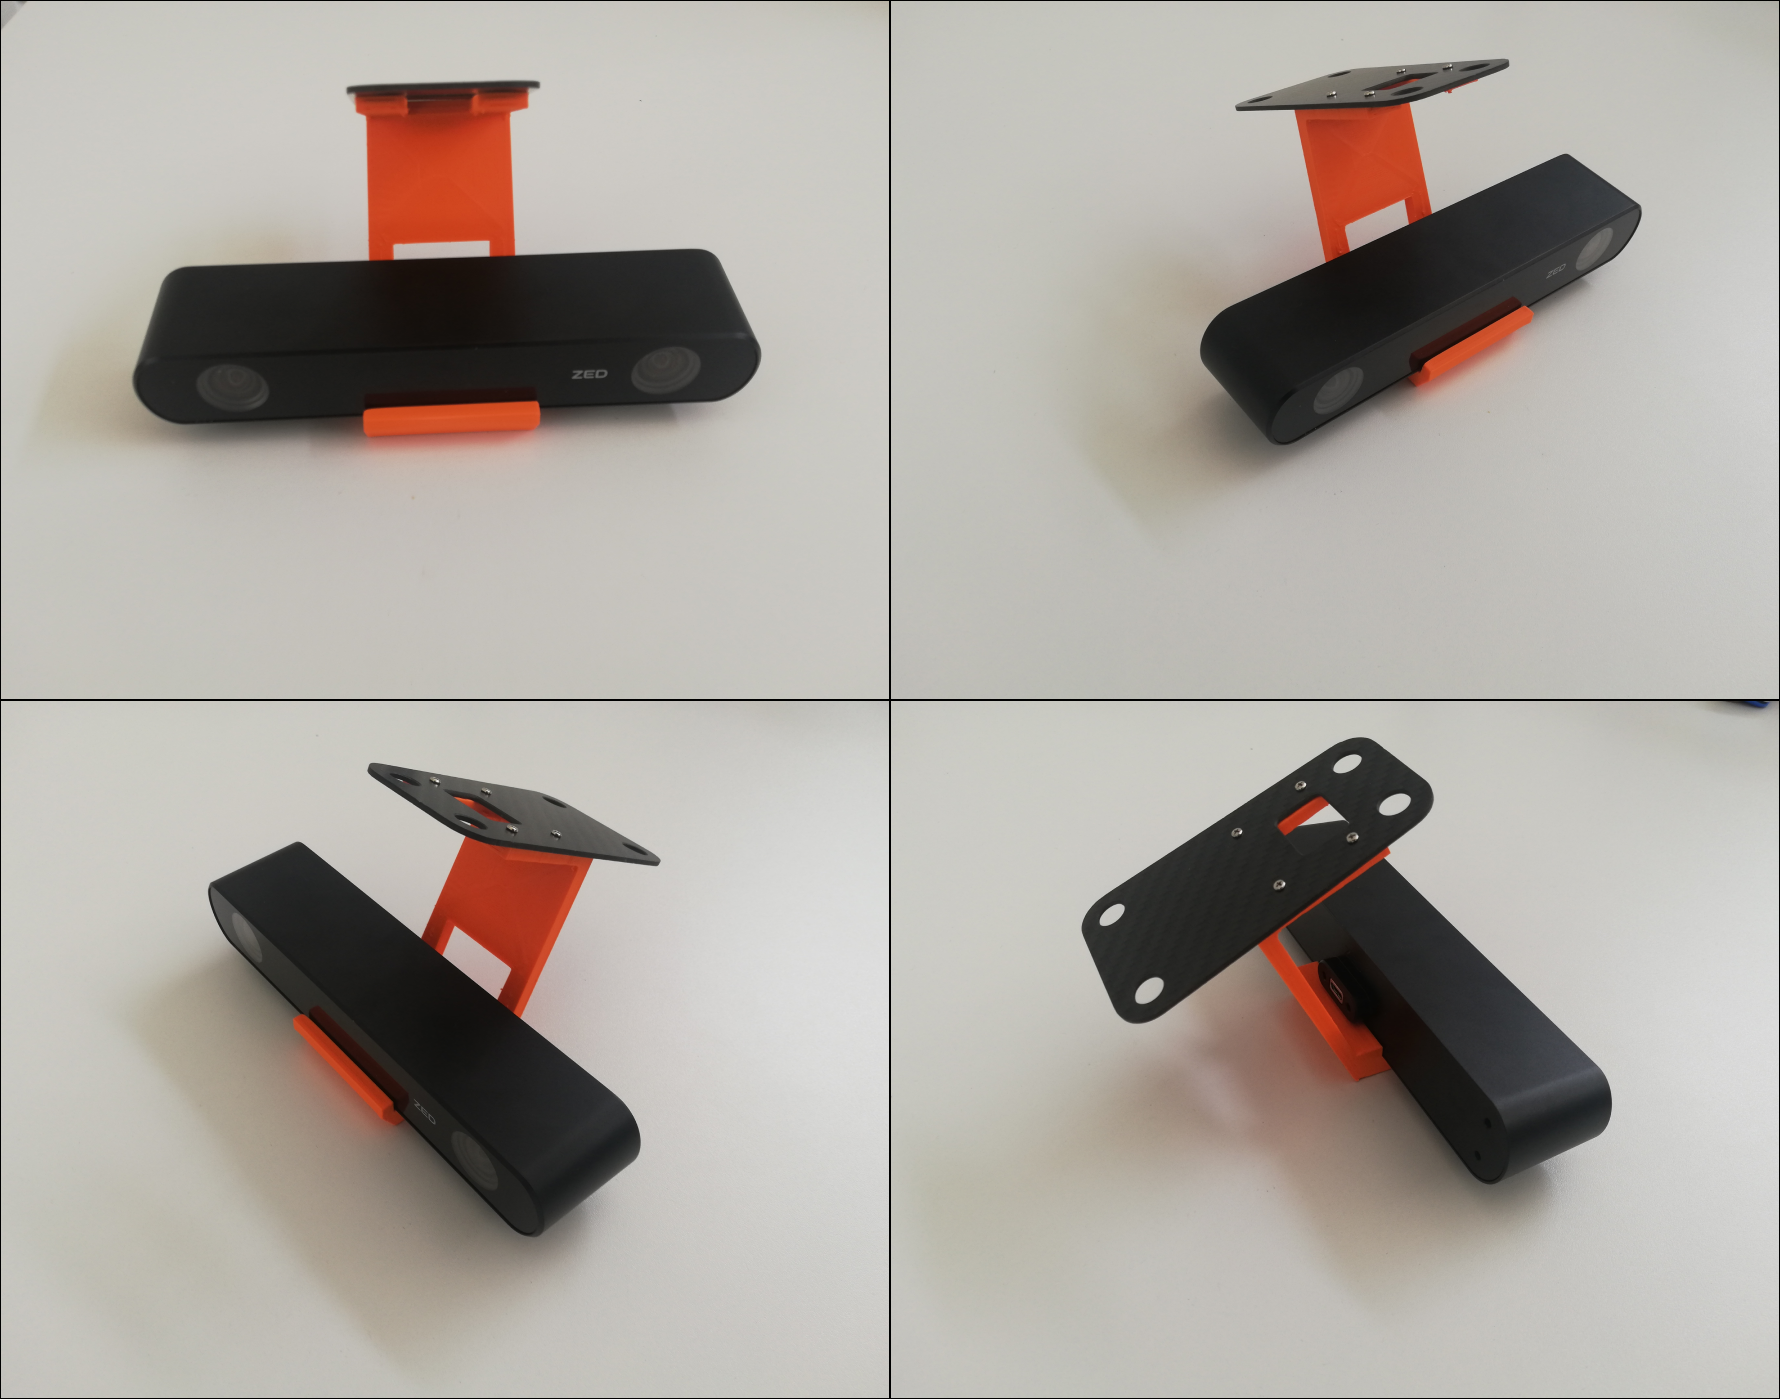
\includegraphics[width=0.6\linewidth]{img/MountPrint}
	\caption{3D-printed camera mount for the purpose of attaching the ZED2i to the Matrice 100. On top of the mount is the connection plate attaching on the drone.}
	\label{fig:custom_parts_mountPrint}
\end{figure}

\section{CAD Software}

This section is going to cover widespread CAD software solution. Nowadays computer aided design is a imperative principle, used in a variety of industries. CAD software improves the efficiency and quality of the design workflow. With free solutions being available, this industry standard has expanded to a clientele reaching from the leading companies to hobbyist creating innovation of the future in the comfort of their homes. Therefor when choosing an apt software, a multiplicity of properties have to be considered.

\subsection{SolidWorks}

SolidWorks being the industry leading CAD solution, it is hard to overlook in a comparison. SolidWorks offers a fast array of functionality for not only CAD, additionally it offers capabilities for computer aided manufacturing. 
The target audience for SolidWorks being experts in the field of modeling and design. Hereby is not only the UI designed to cater more to a clientele which is firm in their understanding of the computer aided design process, but also it offer more in-depth functionalities such as dynamic loading, linear and non-linear analysis and composite materials.\footcite{all3dpSolidWorksVsFusion2021}

\begin{figure}[h]
	\centering
	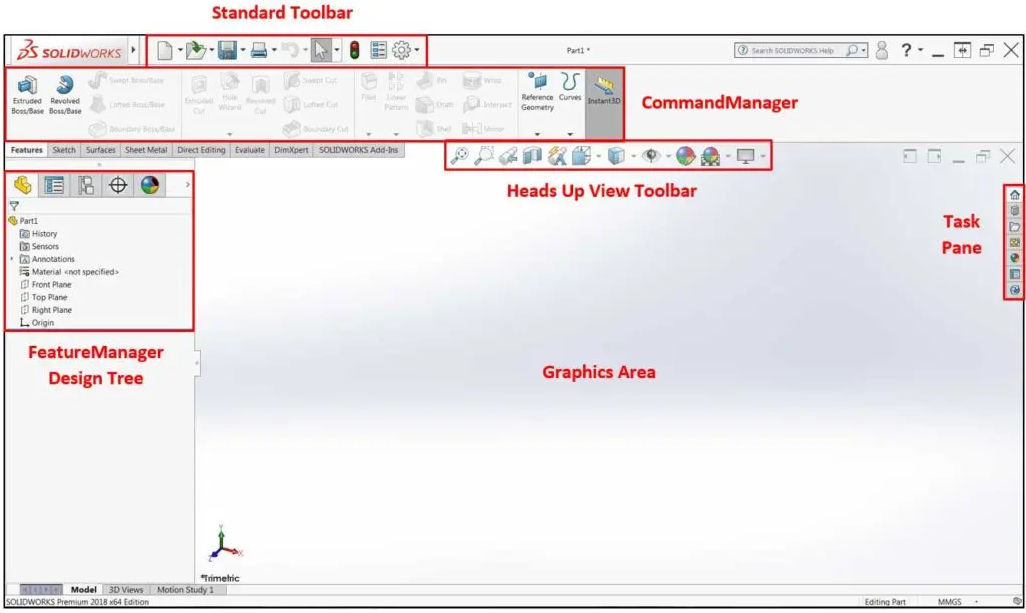
\includegraphics[width=0.6\linewidth]{img/SolidWorksUI}
	\caption{SolidWorks user interface broken up into its different components.\footcite{hawkridgesysUIBSolidWorks2019}}
	\label{fig:custom_parts_solidworks}
\end{figure}


\subsection{Fusion 360}

With Fusion 360 offering a non-commercial, free license option with limited functionality, it is wide spread amongst hobbiest and with its beginner friendly ui design and possibility for an educational license with the majority of the functional scope of the professional license. Features included in the professional subscription that are excluded otherwise are mostly cloud processing options and load and stress simulations.

\begin{table}
	\centering
	\begin{tabular}{ |p{3cm}||p{6cm}|p{3cm}|  }
		\hline
		\multicolumn{3}{|c|}{Fusion 360 Licenses} \\
		\hline
		License & Features & Price\\
		\hline
		Fusion 360 for personal use& Standard design and 3D modeling tools& free\\
		\hline
		Fusion 360& Standard design and 3D modeling tools, plus a fully featured CAM, CAE, and PCB development platform& 495\$ p.a.\\
		\hline
	\end{tabular}
	\caption{An overview of Fusion 360 licenses with their respective capabilities and prices.\footcite{autodeskFusionPersonalNoDate}}
\end{table}

\subsection{Autumn choice}

When comparing the two CAD solution, that are possibilities to be used in the autumn project, the most important characteristic is the user friendliness in respect to the state of knowledge the user already has. Both SolidWorks and Fusion 360 offer more than enough functionality to fulfill the needs of autumn. When looking at the monetary dimension, where for the needed functionality Fusion has no competition with its free license for personal use. Furthermore is the Fusion 360 workflow tailored to simple application, with a small amount of components. SolidWorks follows a assembly based principle, in contrast Fusion 360 is based on a multi-component architecture.\newline
In conclusion due to the limited amount of functionality required from a CAD software in the autumn project, Fusion 360 is being used.

\section{3D-Printing}

This section is going to focus on manufacturing methods available in the autumn project and compare them. Nowadays easy and fast prototyping is made possible with use of 3D-printing technology. 3D-Printing has evolved over the years, away from a science fiction concept, to an widely used tool in part manufacturing, filling the gap left open by the geometrical limitations of conventional methods.\newline
Autumn having an area of competence, split between skills when working with soft- and hardware, it is important to have the means to manufacture custom parts, tailored to the needs of the project. With 3D-Printing being an affordable and accurate technology, in terms of translating virtual concepts to physical object, it is an obvious choice to use for autumn.
When considering using 3D-printing in any kind of project, it is important to think about which method is best fitted for the application.

\subsection{Fused Deposition Modeling}

FDM-printing is the most commonly and wide spread method of 3D-printing. The principle behind fused deposition modeling comprises using an extrusion device to eject a thermoplastic polymer. This polymer is heated to the point of its glass transition and consequentially extruded along a predefined path.\newline

\subsubsection{Movement Variants}

Movement capabilities of 3D-printers differ between two different approaches. Most desktop 3D-printers are Cartesian-style 3D-printers, which means it moves linearly in the x, y and z dimension.
Which parts of the printer move depend on the printer itself, commonly the print-bed moves in the y dimension, while the print-head covers x and the vertical z movement. In Contrast the delta-printing method uses three vertical rods aligned in a triangle shape, to support the print-head and move it per individual movement of sleds, on the vertical rods, connected to the print-head.\footcite{all3dpFDM3DPrinting2020}\newline

\begin{figure}[h]
	\centering
	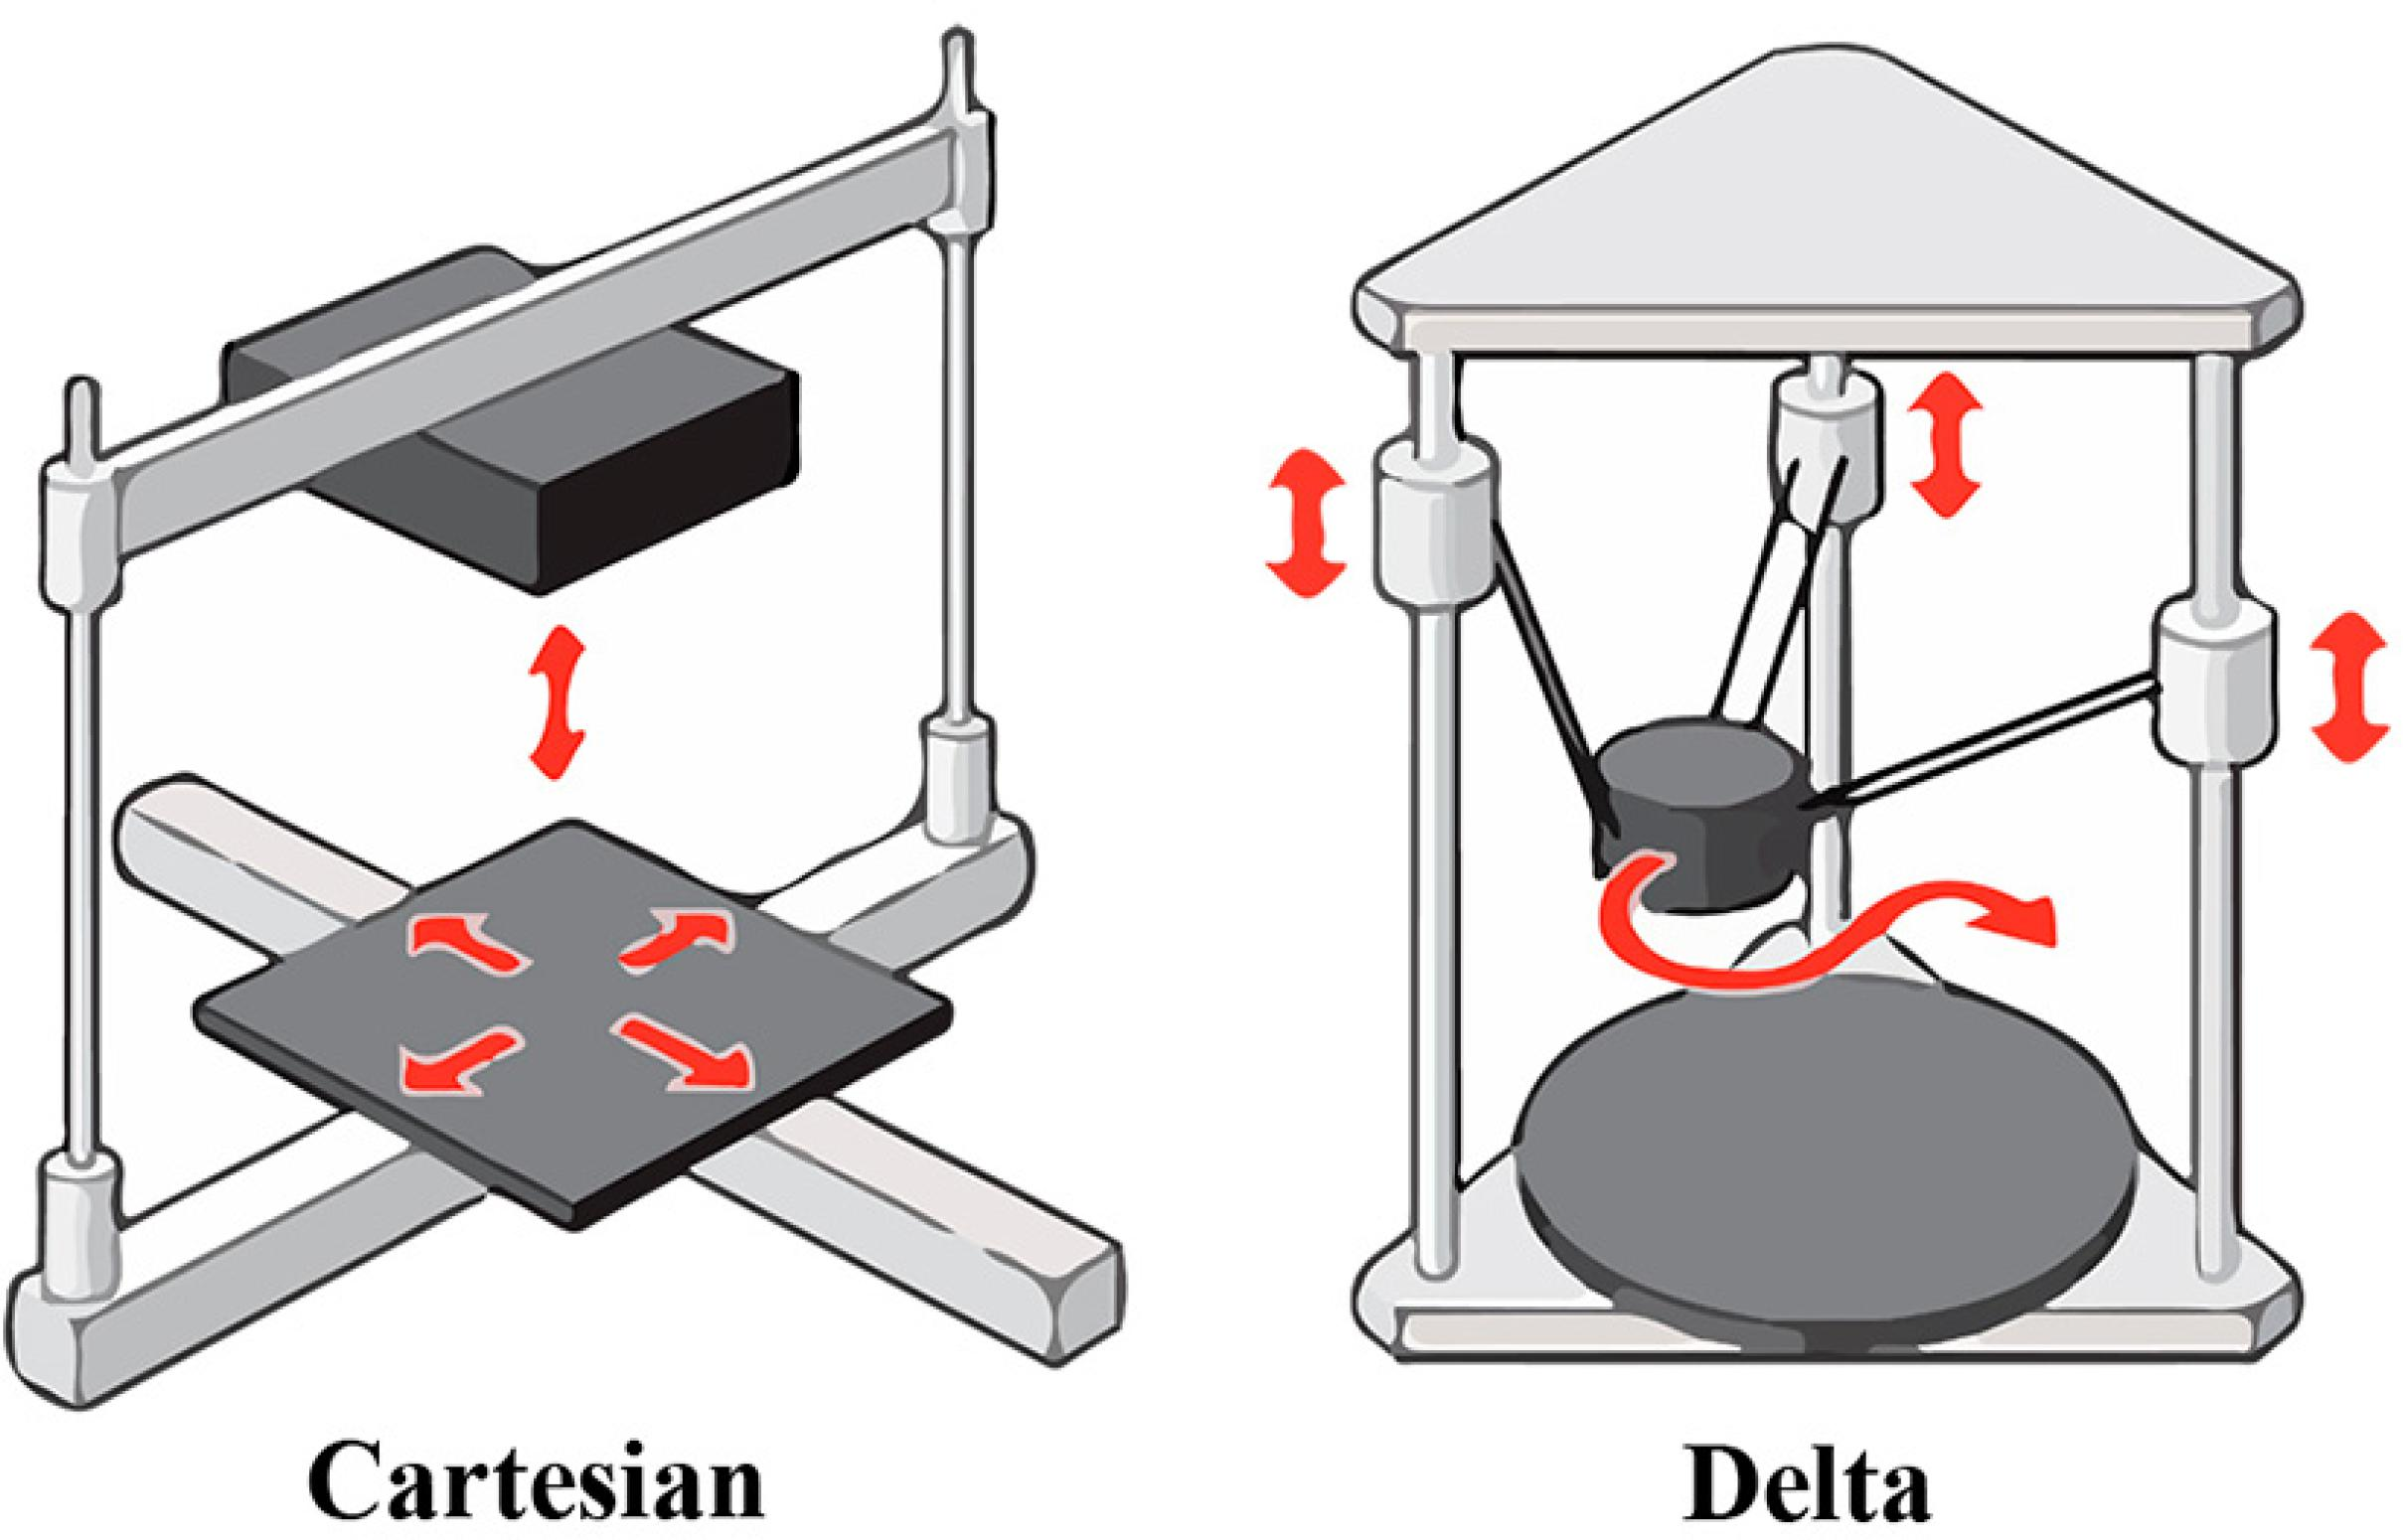
\includegraphics[width=0.6\linewidth]{img/cartesianDeltaPrinting}
	\caption{Portrayal of Cartesian-style and Delta-style 3D-printing.\footcite{Schmitt2017}}
	\label{fig:custom_parts_printerMovement}
\end{figure}

Cartesian-style and Delta-style printers fundamentally contain the same parts. Both printer variants include a print-bed, print-head and stepper-motors, the difference is how they are arranged. Therefor the performance of these printing styles is similar and are more depend on other factors than the movement system. The reason Cartesian-style printers are as popular as they are, is due to the fact that the simpler Cartesian approach is user friendlier and consumes less space, then its delta-style equivalent.\newline

\subsubsection{Main Parts}

In order to be able to distribute the filament in according to the predefined path, calculated by the slicing software, components are needed, namely an extruder, hot-end, and nozzle. The extruder is used the feed the polymer to the print-head. The print-head itself consists of an hot-end and a nozzle, the hot-end is used to heat the thermoplastic polymer to the state of glass transition, after which it is forced through a nozzle an applied to either the print-bed directly or on top another layer.\footcite{all3dpFDM3DPrinting2020}


\begin{figure}[h]
	\centering
	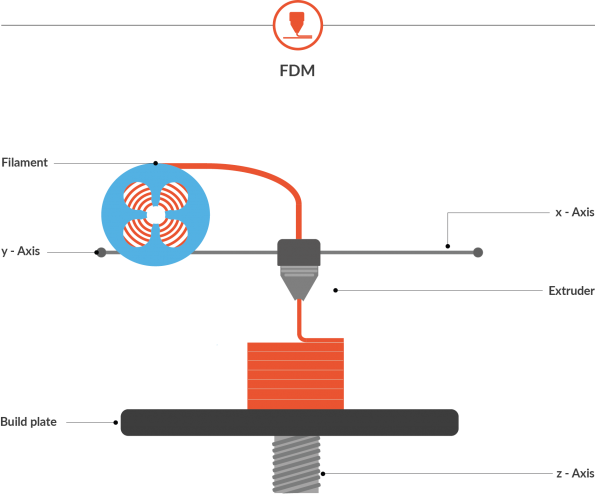
\includegraphics[width=0.6\linewidth]{img/FDM_Principle}
	\caption{Depiction of FDM printer parts, in an Cartesian-style design. \footcite{druckwegeFusedDepositionModelling}}
	\label{fig:custom_parts_fdm_parts}
\end{figure}

\subsubsection{Filament}

The aspect of the filament used for a print, heavily influences the success and usability of a part. The most common filaments include PLA, ABS and Nylon. PLA being the easiest to work with, it is the most frequently used, when needing a more robust material then PLA a suitable polymer would be ABS. Cases where Nylon is used are when highly flexible parts are desired.\footcite{hubsIntroToFDM3DPrintingNoDate}


\subsection{Stereolithography}


	
	\chapter{Conclusion}

\textbf{Author: Fabian Kleinrad} 

\section{Autumn Result}

\subsection{Goal}
The objective of the autumn project is developing a fully autonomous drone capable of generating 3D scans of inaccessible areas. Additionally, it is possible to deploy the drone in regions lacking external localization based on the technologies used. Technologies realizing these features are already available. In contrast to these commercially available solutions, the autumn project aims to accomplish these feats using a low budget approach. 

\subsection{Design choices}
Crucial to the whole operation are means to perceive objects surrounding the drone. To accomplish this, a stereo camera was chosen due the to low cost compared to sensors used for commercial autonomous solutions.\newline
The drone used in the autumn project provides for a wide range of possible sensor configurations and a high payload capacity. This simplified prototyping and helped with the fast iterative approach used in this project. Using a smaller drone would have impeded tests due to the increased complexity of working with compact physical space and smaller weight margins.\newline
To enable computation on the drone itself, an NVIDIA-Jetson TX2 is being employed. This solves the issue of latency problems, which are especially troublesome in processes that need to perform without interruption to guarantee the most optimal results. In the case of the autumn project, such a process would be the continuous mapping of the environment.
\pagebreak
\subsection{Result}
The autumn drone performs mapping using stereo images provided by the stereo camera mounted on the drone. An RRT*-based path-planning algorithm then uses these mapping results to calculate a path originating from the drone's position to an selected end-point. The current position is also provided by the SLAM algorithm in the mapping stage. Using this route information, the drone can be controlled accordingly.
In the current version of the drone, only semi-autonomous flight is supported.Furthermore, due to the lack of testing possibilities and the risk that accompanies testing autonomous drones, flight capabilities were only assessed using user input.

\subsection{Mapping}
With the focus of autumn centring around creating 3D scans of environments, the aspect of mapping is a crucial factor upon which the quality of results depends on.\newline
Mapping was realized by implementing a 3D graph-based SLAM algorithm, supporting stereo imagery. The algorithm determines the current position of the device that provides the images. SLAM generates a point cloud representing the environment the drone explores based on this relative position. All mapping logic is computed on the drone using an NVIDIA-Jetson TX2, which provides enough computational power to ensure the most optimal results. In order to transfer the point cloud data, an access point is being hosted, over which a client may supervise the result. This enables the user to get a real-time view of the model and how it is being constructed. The resulting point-cloud can then be used as reference material in numerous applications.\newline
An example of its utilization would be the basis of a detailed render. In this scenario, it would simplify the process of measuring and conveying the composition into modelling software. The defining structure is already present using a point cloud, and only a few adjustments have to be made.

\subsection{Path-Planning}
Autonomy implies the means to navigate through an environment without external help. In autumn, this is realized using a path-planning algorithm. This algorithm is based on the RRT* algorithm, often employed in high-dimensional and dynamic domains. The algorithm plans a path through either a two-dimensional or three-dimensional representation of the environment surrounding the drone. In autumn, this model is being generated in the mapping phase using the SLAM algorithm.\newline
The path is computed separately from the drone. The reason is that separating the path computation onto an external device allows the drone to work more efficiently and the path-planning algorithm not to be constricted by computational restriction present when computing on the drone itself.\newline
The route is calculated between the drone's current position and a user-defined end-point. If newer mapping data is available, the previously generated path gets checked for possible collisions with newly scanned obstacles. Due to the single-query approach of the RRT algorithm, a new path has to be calculated in the case of the path being invalid.
The resulting path can be visualized for the user alongside the model generated in the mapping phase. This allows for early error detection through a human observer.

\section{Outlook}

\subsection{Current problems}
At current times, fully autonomous flight is not possible with the autumn drone. A significant risk factor in the design is the inability to monitor the space above the drone. This results in problems when using three-dimensional path-planning due to the uncertainty of what lies above. Without that information, the drone is unable to utilize the third dimension, which is the most crucial factor for using a UAV. In autumn, this was solved by focusing on a semi-autonomous approach.  
Another problem is the short battery life-time of the drone, which is due to the size of the drone used in the project. This leads to complications when scanning medium to large environments.  

\subsection{Future solutions}
The modular structure provided by ROS allows the autumn project to be easily implemented using different hardware. It is possible to realize fully autonomous flight using a smaller drone and a simpler two-dimensional lidar for future projects. This results in the loss of three-dimensional mapping capabilities but enables a more reliable and easier environment exploration.\newline 
Furthermore, using ROS, every part of the autumn logic can be used in separate projects where needed.
An example would be using the two-dimensional path-planning algorithm to plan the movement of a ground vehicle. 

\filbreak
	
	
	% Index
	\newpage
	\chapter*{Index}
	\printindex[name]
	\printindex[title]
	
	\printbibliography
	\chapter*{Messbox zur Druckkontrolle}



\begin{center}
{\Large --- Druckgröße kontrollieren! ---}

\bigskip

\Messbox{100}{50} % Angabe der Breite/Hoehe in mm

\bigskip

{\Large --- Diese Seite nach dem Druck entfernen! ---}

\end{center}



\end{document}
